% On découpe ce document complexe en plusieurs sous-fichiers séparés.
% Cela permettra notamment de réarranger les transparents facilement 
% lors de l'élaboration du document.

% La définition de la classe beamer avec tous les styles afférents

\RequirePackage{currfile} 

\documentclass{beamer}

%%%%%%%%%%%%%%%%%%%%%%%%%%%%%%%%%%%%%%%%%
% Beamer Presentation
% LaTeX Template
% Version 1.0 (10/11/12)
%
% This template has been downloaded from:
% http://www.LaTeXTemplates.com
%
% License:
% CC BY-NC-SA 3.0 (http://creativecommons.org/licenses/by-nc-sa/3.0/)
%
%%%%%%%%%%%%%%%%%%%%%%%%%%%%%%%%%%%%%%%%%

%----------------------------------------------------------------------------------------
%	PACKAGES AND THEMES
%----------------------------------------------------------------------------------------




\mode<presentation> {

% The Beamer class comes with a number of default slide themes
% which change the colors and layouts of slides. Below this is a list
% of all the themes, uncomment each in turn to see what they look like.

%\usetheme{default}
%\usetheme{AnnArbor}
%\usetheme{Antibes}
%\usetheme{Bergen}
%\usetheme{Berkeley}
%\usetheme{Berlin}
%\usetheme{Boadilla}
%\usetheme{CambridgeUS}
%\usetheme{Copenhagen}
%\usetheme{Darmstadt}
%\usetheme{Dresden}
%\usetheme{Frankfurt}
%\usetheme{Goettingen}
%\usetheme{Hannover}
%\usetheme{Ilmenau}
%\usetheme{JuanLesPins}
%\usetheme{Luebeck}
%\usetheme{Madrid}		
%\usetheme{Malmoe}
%\usetheme{Marburg}
%\usetheme{Montpellier}
%\usetheme{PaloAlto}
%\usetheme{Pittsburgh}
%\usetheme{Rochester}
%\usetheme{Singapore}
%\usetheme{Szeged}
\usetheme{Warsaw}

% As well as themes, the Beamer class has a number of color themes
% for any slide theme. Uncomment each of these in turn to see how it
% changes the colors of your current slide theme.

%\usecolortheme{albatross}
%\usecolortheme{beaver}
%\usecolortheme{beetle}
%\usecolortheme{crane}
%\usecolortheme{dolphin}
%\usecolortheme{dove}
%\usecolortheme{fly}
%\usecolortheme{lily}
%\usecolortheme{orchid}
%\usecolortheme{rose}
%\usecolortheme{seagull}
%\usecolortheme{seahorse}
\usecolortheme{whale}
%\usecolortheme{wolverine}

%\setbeamertemplate{footline} % To remove the footer line in all slides uncomment this line
%\setbeamertemplate{footline}[frame number] % To replace the footer line in all slides with a simple slide count uncomment this line

%\setbeamertemplate{navigation symbols}{} % To remove the navigation symbols from the bottom of all slides uncomment this line

\setbeamercovered{transparent} % Fait apparaître les animations en grisé (utile pour la conception, mais peut être commenté lors de la remise du document final)

% Pour utiliser une police à empattements partout
\usefonttheme{serif}

% Pour rajouter la numérotation des frames dans les pieds de page
\newcommand*\oldmacro{}%
\let\oldmacro\insertshorttitle%
\renewcommand*\insertshorttitle{%
  \oldmacro\hfill%
  \insertframenumber\,/\,\inserttotalframenumber}

}

\usepackage{graphicx} % Allows including images
\usepackage{booktabs} % Allows the use of \toprule, \midrule and \bottomrule in tables




% Les autres packages utiles  notamment pour le français, les accents ou Python
\usepackage{natbib}         % Pour la bibliographie
\usepackage{url}            % Pour citer les adresses web
\usepackage[T1]{fontenc}    % Encodage des accents
\usepackage[utf8]{inputenc} % Lui aussi
\usepackage[frenchb]{babel} % Pour la traduction française
\usepackage{numprint}       % Histoire que les chiffres soient bien
\usepackage{amsmath}        % La base pour les maths
\usepackage{mathrsfs}       % Quelques symboles supplémentaires
\usepackage{amssymb}        % encore des symboles.
\usepackage{amsfonts}       % Des fontes, eg pour \mathbb.
\usepackage{import}
\usepackage{cancel}
\usepackage{standalone}
%\usepackage[svgnames]{xcolor} % De la couleur
%%% Si jamais vous voulez changer de police: décommentez les trois 
%\usepackage{tgpagella}
%\usepackage{tgadventor}
%\usepackage{inconsolata}
\usepackage{amsmath,amsthm,amssymb,epsfig}
%%% Pour L'utilisation de Python
\usepackage{minted}
\usemintedstyle{friendly}
\usepackage{graphicx} % inclusion des graphiques
\usepackage{wrapfig}  % Dessins dans le texte.
\usepackage{subfigure}
\usepackage{pgfplots, pgfplotstable}
\usepackage[font=footnotesize]{caption}
\usepackage{pgfplots}
\usepackage{tikz}
\usepackage[framemethod=TikZ]{mdframed}
\usepackage{amsmath, amssymb, latexsym}
\usepackage{sidecap}


\usetikzlibrary{decorations.pathreplacing}


\usetikzlibrary{positioning}


\usepackage[font=small,labelfont=bf]{caption}
% Les macros et raccourcis personnels
% Ce fichier contient toutes les macros que vous pouvez avoir envie de définir 
% si vous les utilisez plusieurs fois dans le document.

\PassOptionsToPackage{svgnames}{color}

% Un environnement pour bien présenter le code informatique
\newenvironment{code}{%
\begin{mdframed}[linecolor=green,innerrightmargin=30pt,innerleftmargin=30pt,
backgroundcolor=black!5,
skipabove=10pt,skipbelow=10pt,roundcorner=5pt,
splitbottomskip=6pt,splittopskip=12pt]
}{%
\end{mdframed}
}

% Un raccourci pour composer les unités correctement (en droit)
% Exemple: $v = 10\U{m.s^{-1}}$
\newcommand{\U}[1]{~\mathrm{#1}}

% Les guillemets \ofg{par exemple}
\newcommand{\ofg}[1]{\og{}#1\fg{}}

\def\L{{\mathcal L}}
\def\R{{\mathbb R}}
\def\I{{\mathbb I}}
\def\X{{\mathcal X}}
\def\P{{\mathcal P}}
\def\Y{{\mathcal Y}}

% Le d des dérivées doit être droit: \frac{\dd x}{\dd t}
\newcommand{\dd}{\text{d}}

% La dérivée temporelle, tellement courante en physique, avec les d droits
\newcommand{\ddt}[1]{\frac{\dd #1}{\dd t}}

% Des parenthèses, crochets et accolades qui s'adaptent automatiquement à la 
% taille de ce qu'il y a dedans
\newcommand{\pa}[1]{\left(#1\right)}
\newcommand{\pac}[1]{\left[#1\right]}
\newcommand{\paa}[1]{\left\{#1\right\}}
\captionsetup{justification=centering}
% Un raccourci pour écrire une constante
\newcommand{\cte}{\text{C}^{\text{te}}}

% Pour faire des indices en mode texte (comme les énergie potentielles)
\newcommand{\e}[1]{_{\text{#1}}}

% Le produit vectoriel a un nom bizarre:
\newcommand{\vectoriel}{\wedge}

%%%% debut macro %%%%
\makeatletter
\renewcommand{\thefigure}{\ifnum \c@section>\z@ \thesection.\fi
 \@arabic\c@figure}
\@addtoreset{figure}{section}
\makeatother


\setbeamertemplate{caption}[numbered]
%%%% fin macro %%%%

% On définit le titre et l'auteur du document

% L'argument optionnel (entre crochets) donne le titre qui sera mis sur chaque slide
\title[TIPE : DPI]{Détecteur des Plaques d’Immatriculation (DPI) : Application dans un parking}
\author{Ilyas \textsc{Moutawwakil} : BE026T} % Votre nom
% L'épreuve (car on n'a pas le droit de signaler sa provenance à un concours) (là encore, l'argument optionnel apparaît sur chaque slide)
\institute[TIPE]{Épreuve de TIPE}
\date{Session 2019} 
\pgfplotsset{compat=1.15}
% On démarre le document proprement dit
\begin{document}

% La page de titre et la table des matières
% Rien d'autre à faire qu'afficher le titre
\begin{frame}
\titlepage 
\end{frame}


% La table des matières utilise ce que vous donnez aux commandes \section et 
% \subsection tout au long de la présentation.
\begin{frame}
\frametitle{Plan de l'exposé} 
\tableofcontents 
\end{frame}


% La première grande partie: introduction du sujet
% Titre de la premiere partie

\section{Introduction au système : DPI}
%%%%%%%%%%%%%%%%%%%%%%%%%%%%%%%%%%%%%%%%%%%%%%%%
% Première diapo
%%%%%%%%%%%%%%%%%%%%%%%%%%%%%%%%%%%%%%%%%%%%%%%%
\begin{frame}
\frametitle{Introduction au système : DPI}
\framesubtitle{Problème}

\begin{itemize}
	\item	<1->	Le contrôle d'accès aux espaces privés.
	%\item	<2->	Contraintes : Luminosité, Bruit, Angle d'inclinaison ...
\end{itemize}

\begin{figure}
\begin{overprint}
	\onslide<1>\centering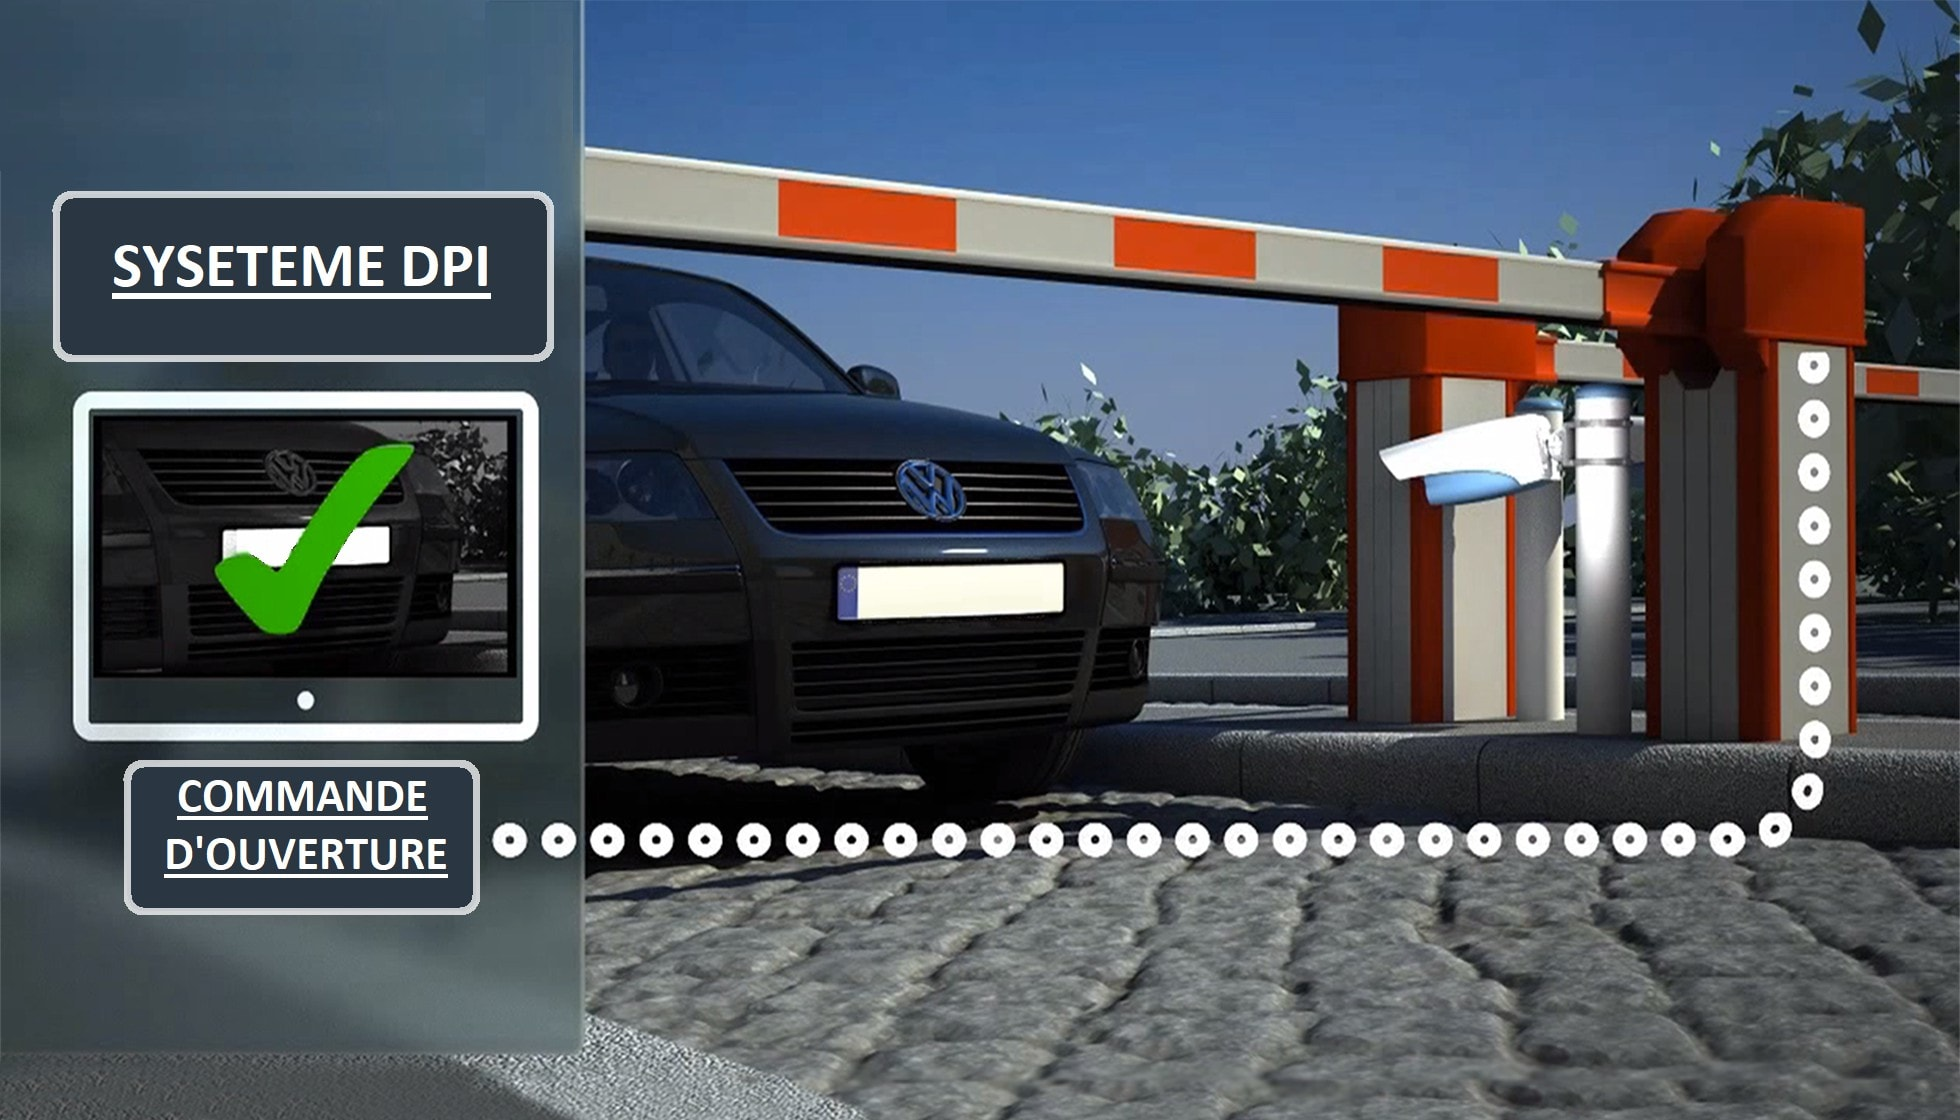
\includegraphics[width=0.7\linewidth]{figures/DPI.PNG}\caption{Exemple d'application du système}
	%\onslide<2>\centering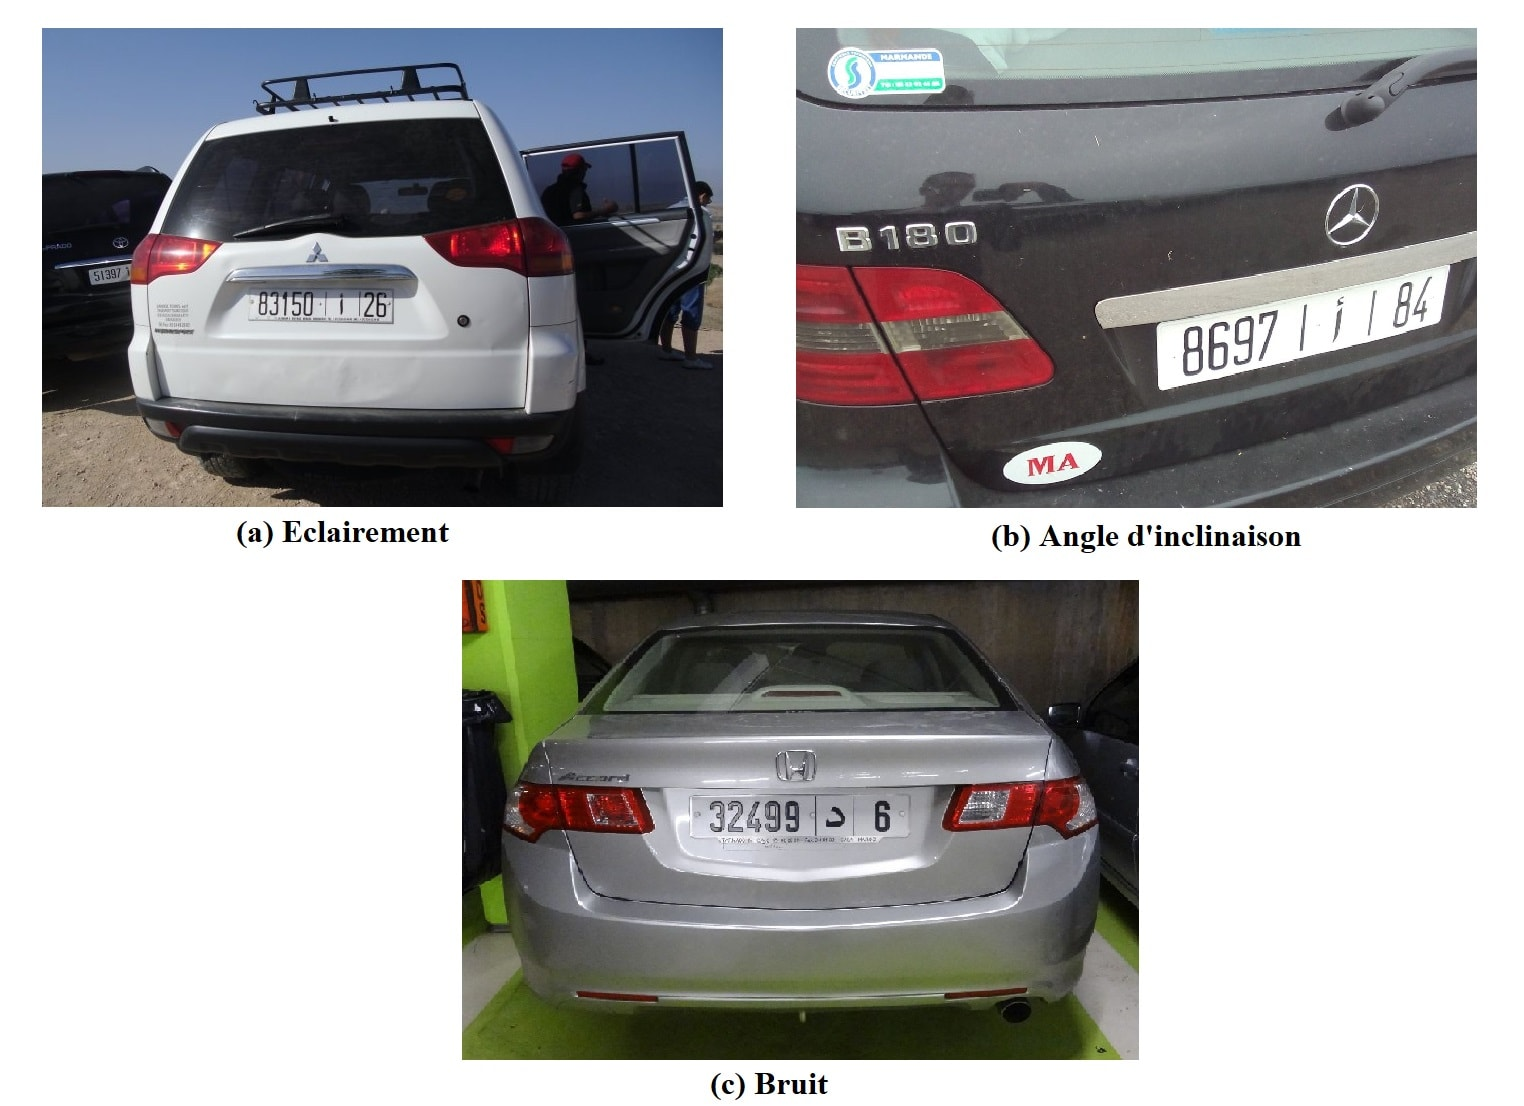
\includegraphics[width=0.6\linewidth]{figures/Contraintes.PNG}\caption{Contraintes de détection}
\end{overprint}
\end{figure}
	
\end{frame}


%%%%%%%%%%%%%%%%%%%%%%%%%%%%%%%%%%%%%%%%%%%%%%%%
% Troisième diapo
%%%%%%%%%%%%%%%%%%%%%%%%%%%%%%%%%%%%%%%%%%%%%%%%
\begin{frame}
\frametitle{Introduction au système : DPI}
\framesubtitle{Solution}

\begin{itemize}
	\item	<1>	Un processus simple et dynamique assurant une detection rapide et précise des plaques !
	\begin{figure}
	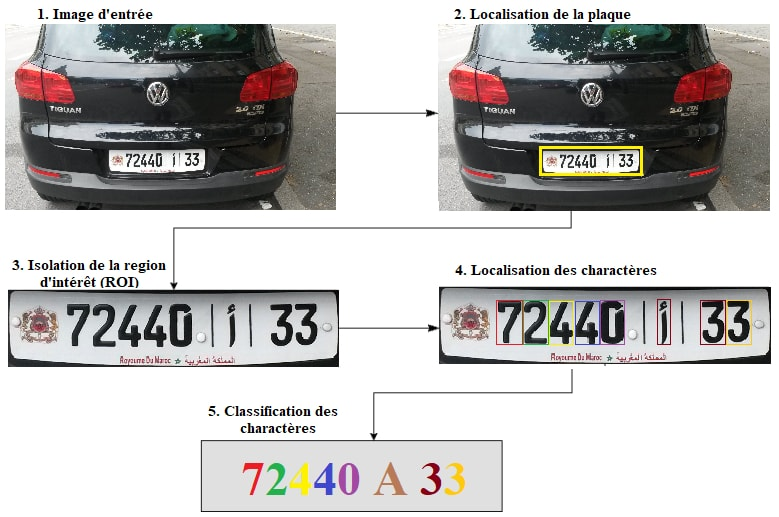
\includegraphics[width=0.7\linewidth]{figures/Process.PNG}\caption{Le processus de reconnaissance optimal}
	\end{figure}
\end{itemize}

\end{frame}

%%%%%%%%%%%%%%%%%%%%%%%%%%%%%%%%%%%%%%%%%%%%%%%%
% Deuxième diapo
%%%%%%%%%%%%%%%%%%%%%%%%%%%%%%%%%%%%%%%%%%%%%%%%
\begin{frame}
\frametitle{Introduction au système : DPI}
\framesubtitle{Analyse Fonctionnelle}
\captionsetup{justification=centering}

\begin{figure}
    \centering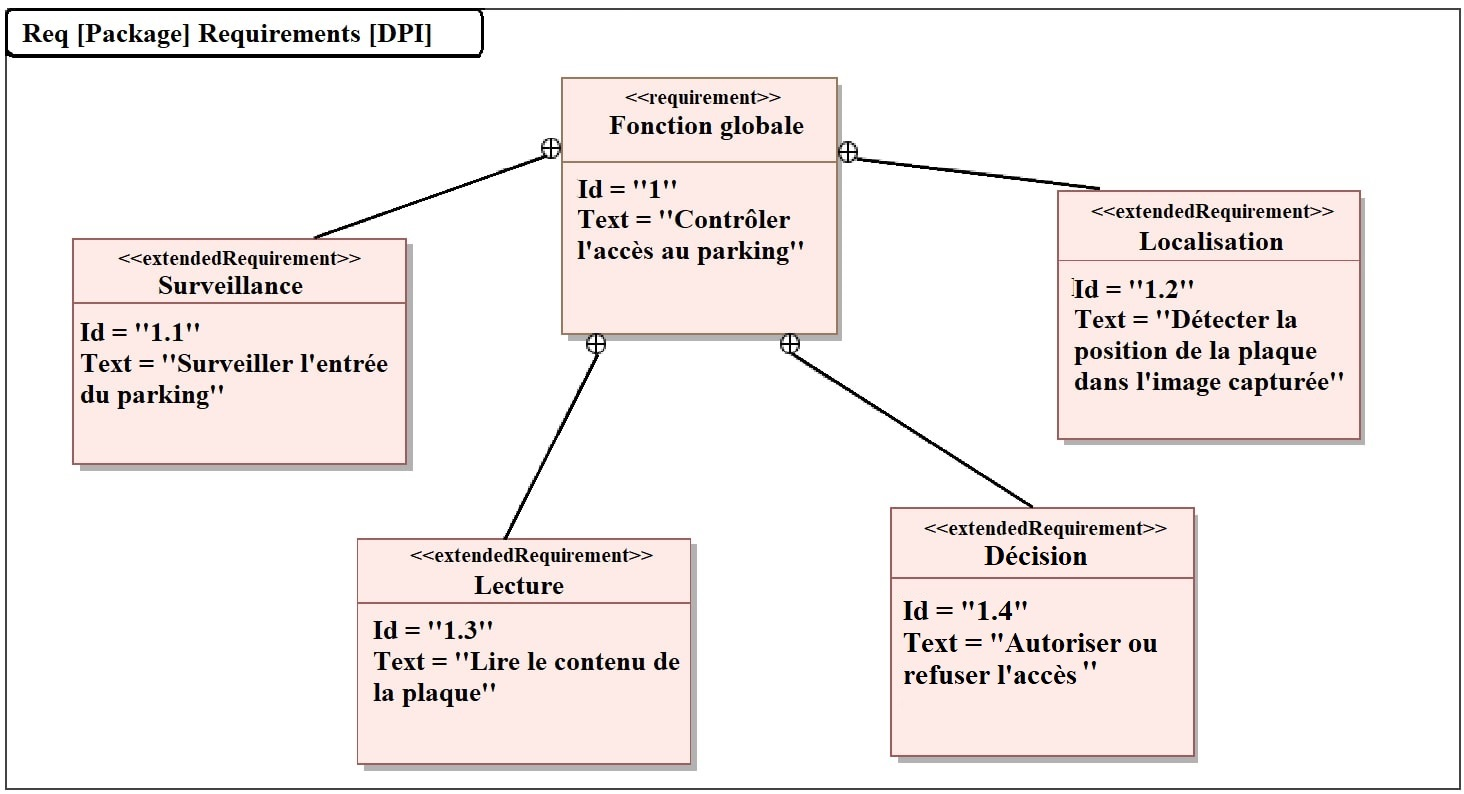
\includegraphics[width=0.9\linewidth]{figures/Req.PNG}\caption{Diagramme d'exigences}
\end{figure}
\end{frame}
%%%%%%%%%%%%%%%%%%%%%%%%%%%%%%%%%%%%%%%%%%%%%%%%
% Quatième diapo
%%%%%%%%%%%%%%%%%%%%%%%%%%%%%%%%%%%%%%%%%%%%%%%%
\begin{frame}
\frametitle{Introduction au système : DPI}
\framesubtitle{Une approche}

\begin{itemize}
    \item	<1>    Développer des algorithmes basés sur les nouvelles techniques d'apprentissage profond pour la localisation et la reconnaissance.
\end{itemize}
\begin{figure}
    
\includegraphics[width=1\linewidth]{figures/Biblio.PNG}\caption{Les trois bibliothèques essentielles}
\end{figure}
        
\end{frame}

% La 2e partie: Le point de vue de la relativité restreinte
% Titre de la partie
\section{La théorie des réseaux de neurones artificiels}

%%%%%%%%%%%%%%%%%%%%%%%%%%%%%%%%%%%%%%%%%%%%%%%%
% Première diapo
%%%%%%%%%%%%%%%%%%%%%%%%%%%%%%%%%%%%%%%%%%%%%%%%

\begin{frame}
\frametitle{Réseau de neurones artificiels}
\framesubtitle{Perceptron}
\begin{columns}
    \begin{column}{6cm}
        \begin{itemize}
            \item<1->   Le perceptron : Une fonction à paramètres ajustables.
        \end{itemize}
        \centering
        \begin{figure}
        \includestandalone[width=1.0\textwidth]{preambule/perceptron}
        \end{figure}
        $$S=A(\sum_{i=1}^{n} (e_i . p_i) + b)$$
    \end{column}
\begin{column}{6cm}
    \begin{itemize}
    \item<2->La fonction d'activation A.
    \begin{itemize}
    \item<2->Heaviside:
    \[A(x) =\begin{cases}
                                   0 & \text{if $x\leqslant0$} \\
                                   1 & \text{if $x>0$}
            \end{cases}\]
    \item<2->Sigmoid : 
    $$ A(x) = \frac{1}{1+exp(-x)}$$
    \item<2->RELU:
    \[A(x) =\begin{cases}
                                   0 & \text{if $x\leqslant0$} \\
                                   x & \text{if $x>0$}
            \end{cases}\]
    \end{itemize}
    \end{itemize}
\end{column}
\end{columns}
\end{frame}


%%%%%%%%%%%%%%%%%%%%%%%%%%%%%%%%%%%%%%%%%%%%%%%%
% Deuxième diapo
%%%%%%%%%%%%%%%%%%%%%%%%%%%%%%%%%%%%%%%%%%%%%%%%
\begin{frame}
\frametitle{Réseau de neurones artificiels}
\framesubtitle{Réseau profond}
\begin{itemize}
    \item<1->   Le théorème d'approximation universelle.
    
    %the so called Universal approximation theorem, proved by Cybenko in 1989 and generalized by various people in the 1990s. It basically says that a shallow neural network (with 1 hidden layer) can approximate any function, i.e. can in principle learn anything. This is true for various nonlinear activation functions, including rectified linear units that most neural networks are using today
    %If so, then why is everybody using deep nets?
    
    \item<2->   Pourquoi un réseau multi-couches (Profond) ?
\end{itemize}
\centering
\begin{figure}
    \begin{overprint}
        \onslide<1>\centering\includestandalone[width=0.6\textwidth]{preambule/one_layer_perceptron}\caption{Réseau
        mono-couche}
        \onslide<2>\centering\includestandalone[width=0.6\textwidth]{preambule/mul_layer_perceptron}\caption{Réseau multi--couche}
    \end{overprint}
\end{figure}
\end{frame}

%%%%%%%%%%%%%%%%%%%%%%%%%%%%%%%%%%%%%%%%%%%%%%%%
% Troisième diapo
%%%%%%%%%%%%%%%%%%%%%%%%%%%%%%%%%%%%%%%%%%%%%%%%
\begin{frame}
\frametitle{Algorithme d'apprentisage}
\framesubtitle{Modélisation du problème}
\begin{itemize}
    \item<1->   Base de données annotées : ${(x_1,y_1), \ldots,(x_n,y_n)}$ .
    \item<2->   Fonction paramétrée : $f_P:\X \to \Y$ .
    \item<2->   Fonctions de coût : $ \L_i:\P\to\R \quad ; \quad  \L(P)=\frac{1}{n}\sum_{i=1}^n \L_i(P)$ .
\end{itemize}

\begin{columns}
    \begin{column}{6cm}
        %\begin{itemize}
            % Une fonction generalement continue vectoriell : Le cout d'une maison en fonction de sa surface, position et durée de construction.
            %\item<4->   Moyenne d'Erreur Carrée
        %\end{itemize}
        \begin{figure}
        \begin{overprint}
            \onslide<1-2>\centering\includestandalone[width=0.6\textwidth]{preambule/linear_reg_data}\caption{Problème de regréssion}
            \onslide<3>\centering\includestandalone[width=0.6\textwidth]{preambule/linear_reg_func}\caption{Fonction de régression}
        \end{overprint}
    \end{figure}
    \end{column}
    \begin{column}{6cm}
        %\begin{itemize}
            % Une fonction generalement discontinue qui arrive dans N : Le chiffre ecrit sur une image 28*28 (Probleme MNIST)
            %\item<4->   Entropie Croisée Binaire
        %\end{itemize}
        \begin{figure}
        \begin{overprint}
            \onslide<1-2>\centering\includestandalone[width=0.6\textwidth]{preambule/class_data}\caption{Problème de classification}
            \onslide<3>\centering\includestandalone[width=0.6\textwidth]{preambule/class_borders}\caption{Frontière de décision}
        \end{overprint}
        \end{figure}
    \end{column}
\end{columns}
\end{frame}

%%%%%%%%%%%%%%%%%%%%%%%%%%%%%%%%%%%%%%%%%%%%%%%%
% Quatrième diapo
%%%%%%%%%%%%%%%%%%%%%%%%%%%%%%%%%%%%%%%%%%%%%%%%
\begin{frame}
\frametitle{Algorithme d'apprentisage}
\framesubtitle{La minimisation d'une fonction}
\begin{columns}
    \begin{column}{6cm}
        \begin{itemize}
            \item<1->   $\L$ est une fonction définie sur l'espace de poids.
            \item<2->   Objectif : Trouver la valeur de $P^{*}$ qui minimise $\L$.
            \item<3->   Méthode : Descente de gradient $$ P^{(i+1)}=P^{(i)} - {\eta}_i \nabla \L (P^{(i)}) $$
            % La base de donnees etant fixee, la dimension de l'espace des poids est egale au nombre de parametres Pij
        \end{itemize}
    \end{column}
    \begin{column}{6cm}
    \begin{figure}
        \begin{overprint}
            \onslide<1>\includestandalone[width=1\textwidth]{preambule/loss_3d}\caption{La forme de $\L$ : cas de deux paramètres}
            \onslide<2>\includestandalone[width=1\textwidth]{preambule/loss_minimum}\caption{Le minimum de $\L$ : cas de deux paramètres}
            \onslide<3>\includestandalone[width=0.8\textwidth]{preambule/loss_proj_grad_desc}\caption{Le chemin de descente}
        \end{overprint}
    \end{figure}
    \end{column}
\end{columns}
\end{frame}

% La 3e partie: Le point de vue de la relativité générale
% Le titre de la partie
\section{La pratique des réseaux de neurones artificiels}

%%%%%%%%%%%%%%%%%%%%%%%%%%%%%%%%%%%%%%%%%%%%%%%%
% Première diapo
%%%%%%%%%%%%%%%%%%%%%%%%%%%%%%%%%%%%%%%%%%%%%%%%

\begin{frame}
\frametitle{Création de la base de données}
\framesubtitle{Données réelles}

\begin{columns}
\begin{column}{6.8cm}
    \begin{itemize}
        \item<1->   Chercher des images sur Internet.
        \begin{itemize}
            \item<1->   Google et quelques sites web.
        \end{itemize}
        %Quantité trés faible d'images sur internet
        \item<1->   Prendre des photos de la rue.
        \begin{itemize}
            \item<1->   Parkings publics.
        \end{itemize}
        %Problèmes d'autorisation et de nécéssité d'explication
        \item<2->   Écire un programme d'annotation.
        %Permettant l'annotation en des fichiers texte contenant les coordonnées des plaques
        \item<2->   Annoter les images collectées.
    \end{itemize}
\end{column}
\begin{column}{6cm}
    \begin{figure}
        \begin{overprint}
            \captionsetup{justification=centering}
            \onslide<1>\centering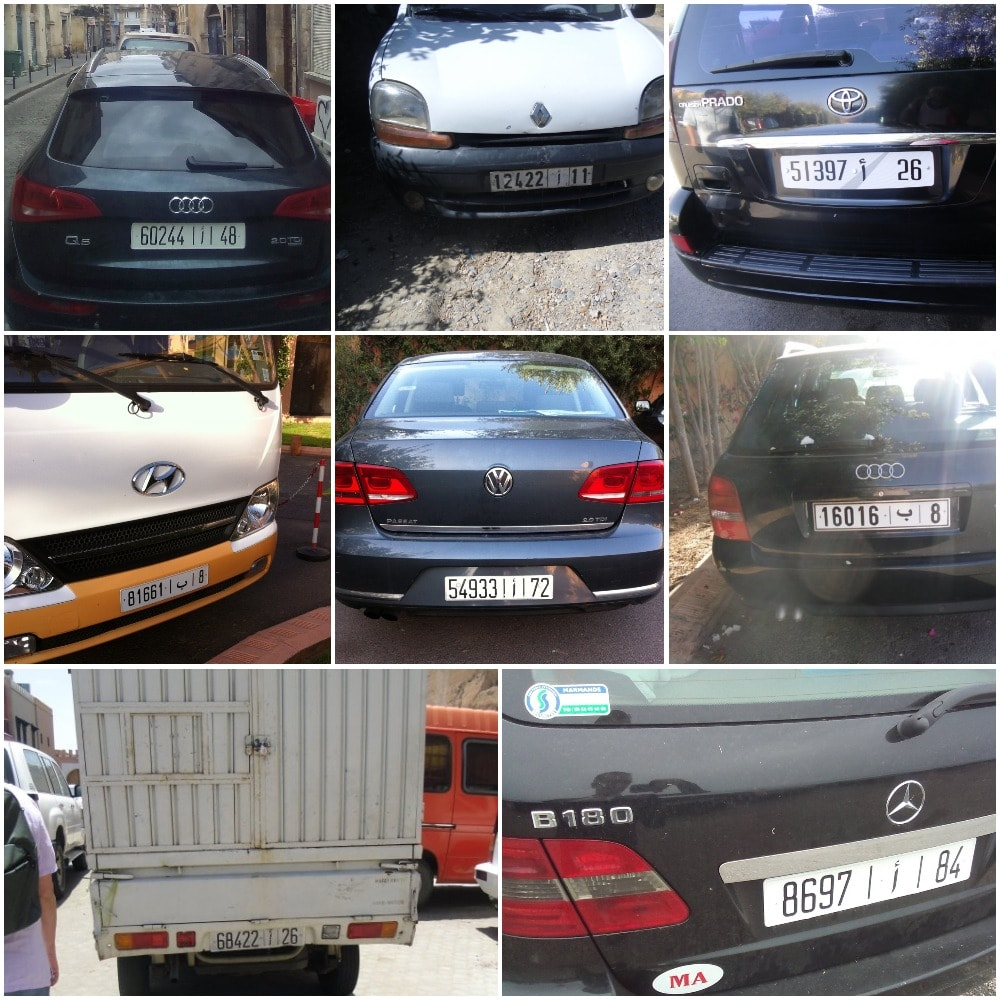
\includegraphics[width=0.8\textwidth]{figures/Data_real.PNG}\caption{Exemples d'images collectées}
            \onslide<2>\centering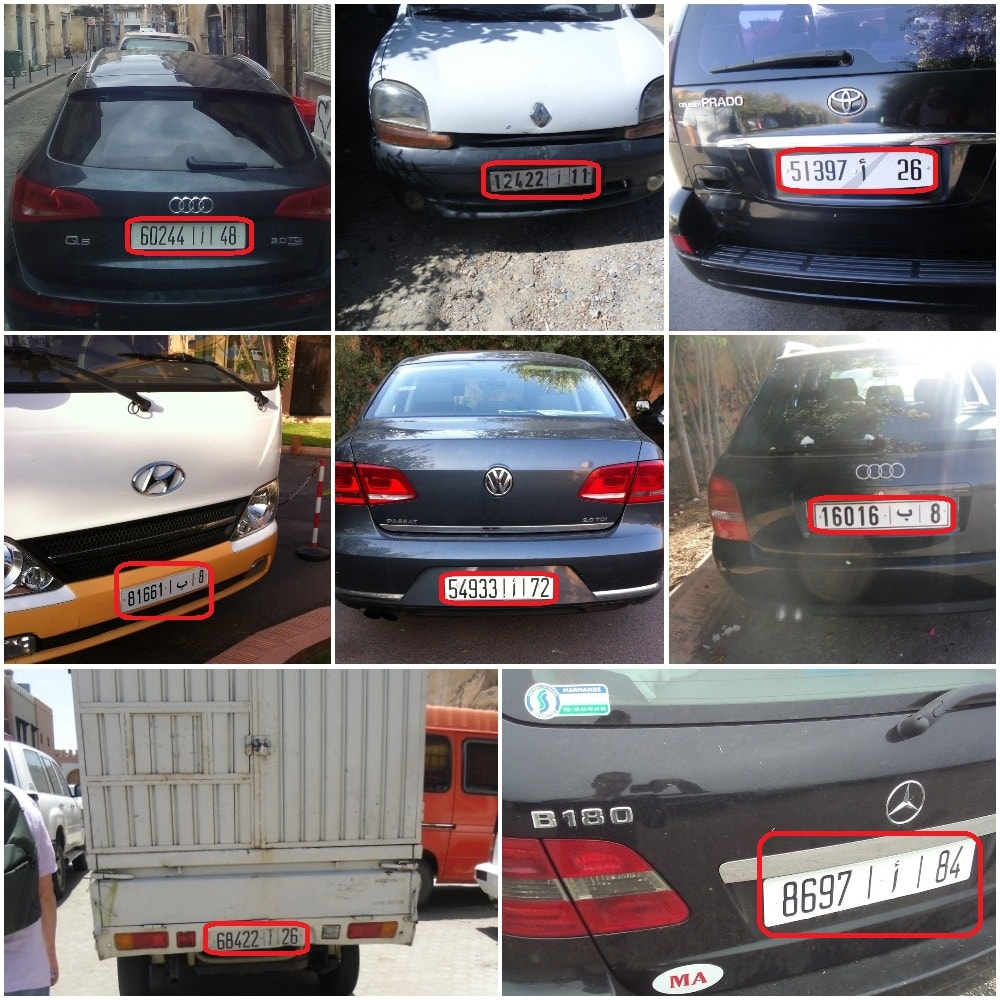
\includegraphics[width=0.8\textwidth]{figures/Data_ann.PNG}\caption{Exemples d'images annotées}
        \end{overprint}
    \end{figure}
\end{column}
\end{columns}

\end{frame}


%%%%%%%%%%%%%%%%%%%%%%%%%%%%%%%%%%%%%%%%%%%%%%%%
% Deuxième diapo
%%%%%%%%%%%%%%%%%%%%%%%%%%%%%%%%%%%%%%%%%%%%%%%%

\begin{frame}
\frametitle{Création de la base de données}
\framesubtitle{Données synthétisées}

\begin{columns}
\begin{column}{6cm}
    \begin{itemize}
        \item<1->   Analyser les caractéristiques des plaques marocaines.
        \item<2->   Trouver une base de données d'images sans plaques.
        \item<3->   Écrire un programme qui génère des données annotées.
        \item<4->   Analyser et optimiser la qualité des données générées.
    \end{itemize}
\end{column}
\begin{column}{6cm}
    \begin{figure}
        \begin{overprint}
            \onslide<1>\centering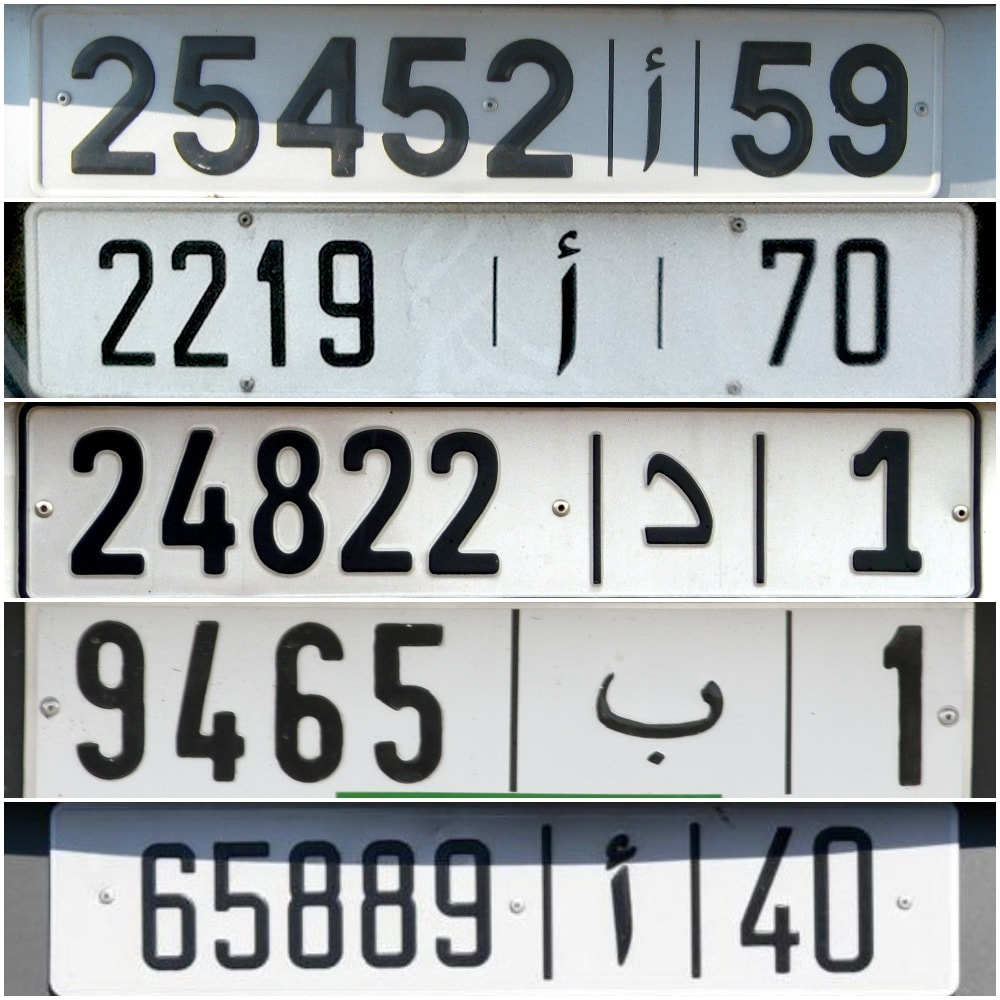
\includegraphics[width=0.8\textwidth]{figures/Plaques.PNG}\caption{Exemples de plaques maroccaines}
            \onslide<2>\centering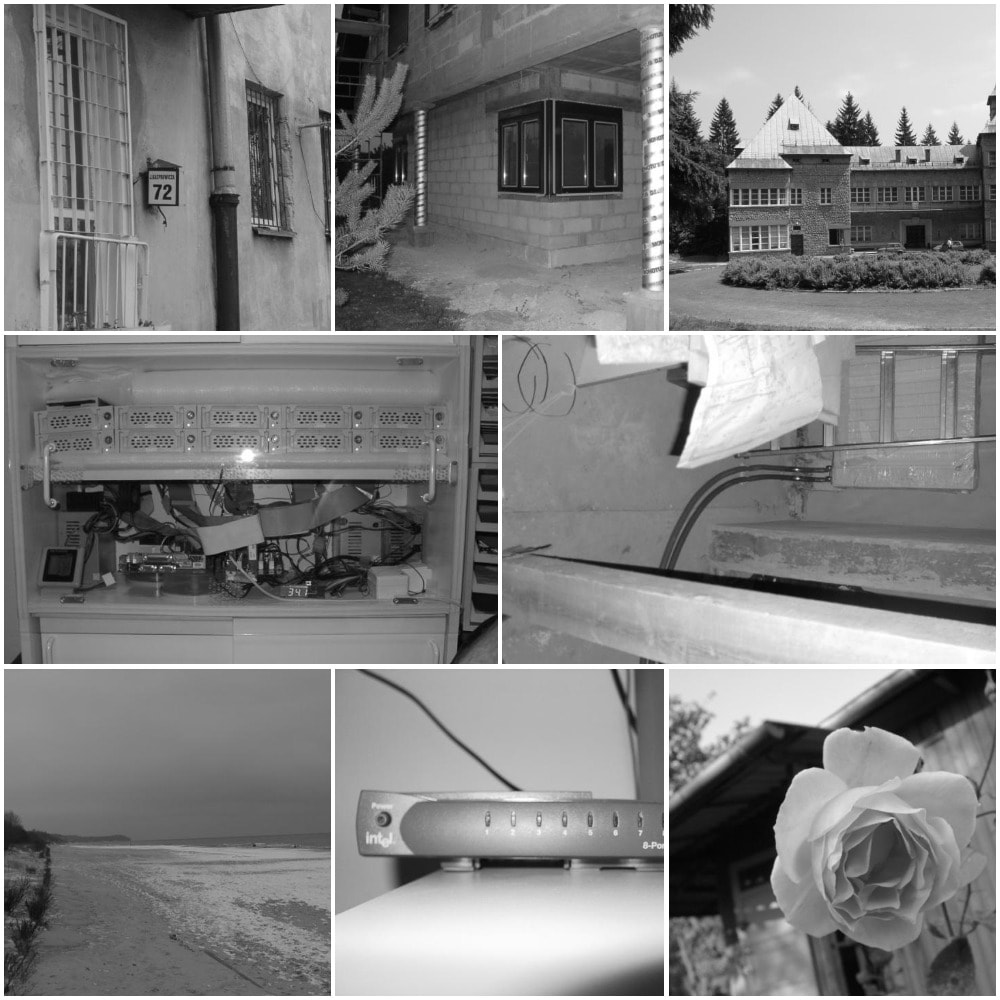
\includegraphics[width=0.8\textwidth]{figures/SUN_data.PNG}\caption{Exemples d'images sans plaques}
            \onslide<3>\centering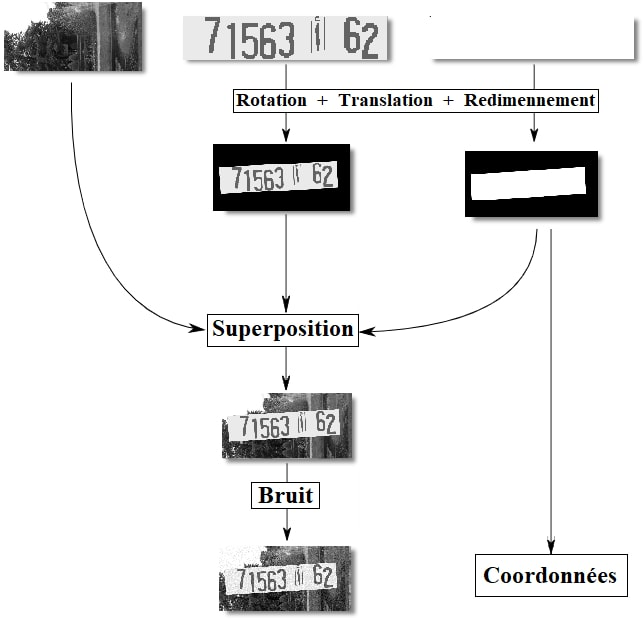
\includegraphics[width=0.8\textwidth]{figures/Gen_process.PNG}\caption{Le processus des génération de données annotées}
            \onslide<4>\centering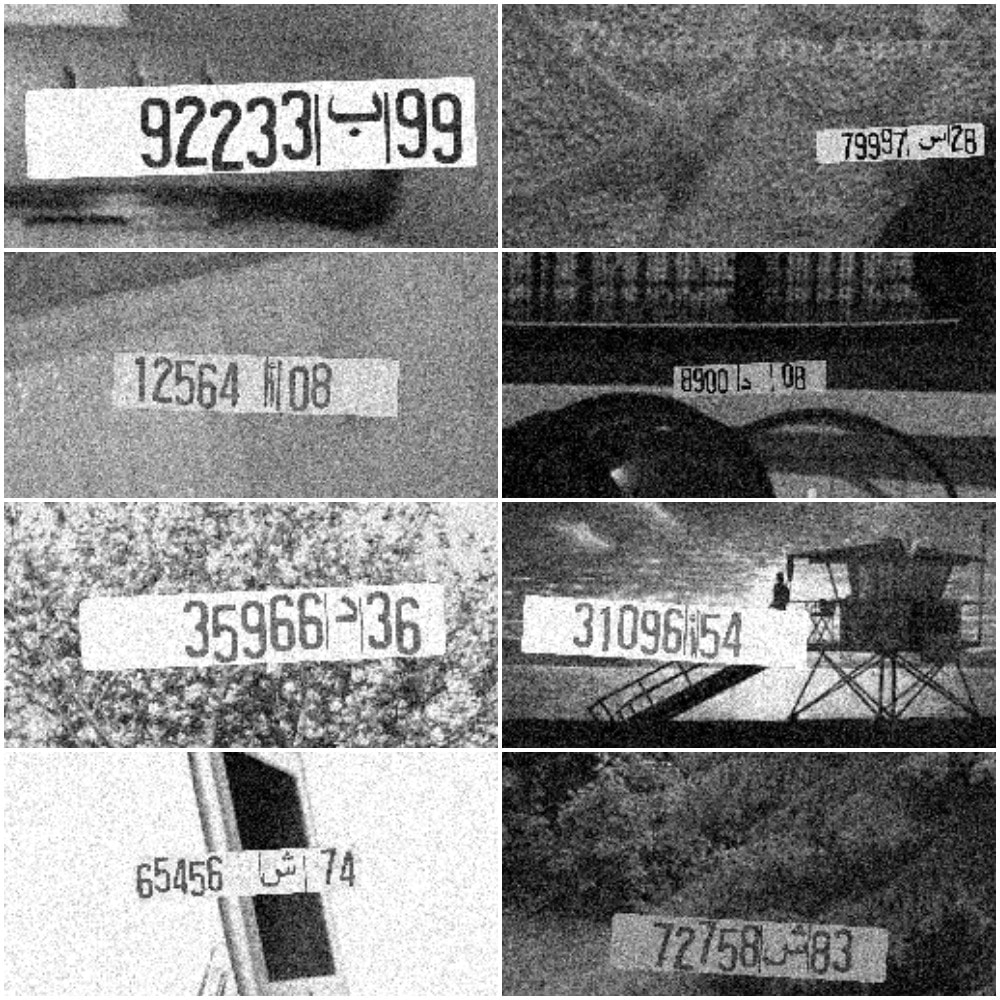
\includegraphics[width=0.8\textwidth]{figures/Data_gen.PNG}\caption{Exemples des données générées}
        \end{overprint}
    \end{figure}
\end{column}
\end{columns}
\end{frame}


%%%%%%%%%%%%%%%%%%%%%%%%%%%%%%%%%%%%%%%%%%%%%%%%
% Troisième diapo
%%%%%%%%%%%%%%%%%%%%%%%%%%%%%%%%%%%%%%%%%%%%%%%%

\begin{frame}
\frametitle{Création de la base de données}
\framesubtitle{Comparaison entre bases de données}
\begin{table}

\begin{tabular}{c|c|c|c}
    Type de données  &  Moyenne  &  Ecart type &  Coefficient de variation \\
    \hline
    Générées         &  126      &  32.71      &  3.86  \\
    Réelles          &  97.84    &  24.79      &  3.94
\end{tabular}
\end{table}
\centering
\begin{figure}
    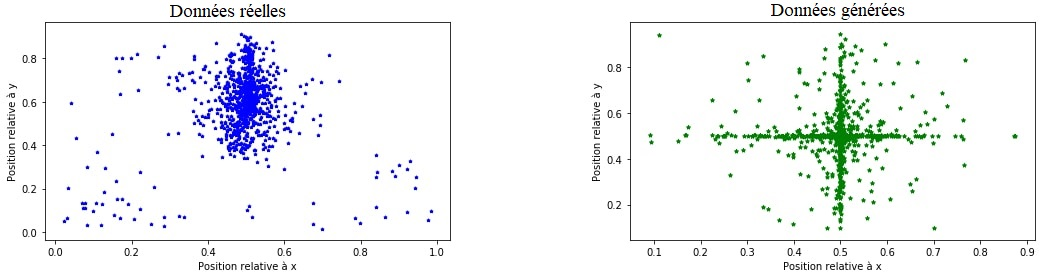
\includegraphics[width=1\textwidth]{figures/Data_dispers.PNG}\caption{Dispersion des centres des plaques}
\end{figure}
\end{frame}

%%%%%%%%%%%%%%%%%%%%%%%%%%%%%%%%%%%%%%%%%%%%%%%%
% Quatrième diapo
%%%%%%%%%%%%%%%%%%%%%%%%%%%%%%%%%%%%%%%%%%%%%%%%

\begin{frame}
\frametitle{Création du réseau de neurones}
\framesubtitle{Un problème de régression ?}
\begin{columns}
\begin{column}{6.5cm}
    \begin{itemize}
        \item<1->   Un model simple de prédiction.
        \item<2->   Prédictions érronées.
        \item<2->   Problème de "Surapprentissage" .
    \end{itemize}
\end{column}
\begin{column}{6cm}
    \begin{figure}
        \begin{overprint}
            \onslide<1>\centering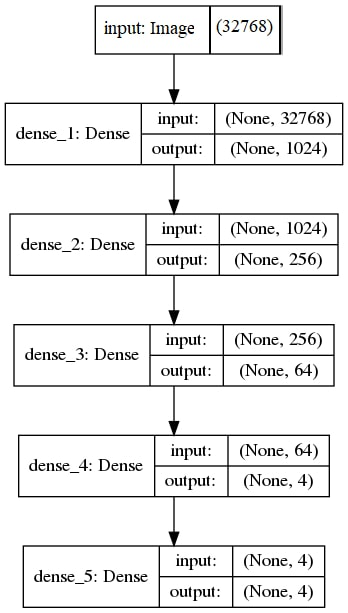
\includegraphics[width=0.5\textwidth]{figures/Model_1.PNG}\caption{Model de régression}
            \onslide<2>\centering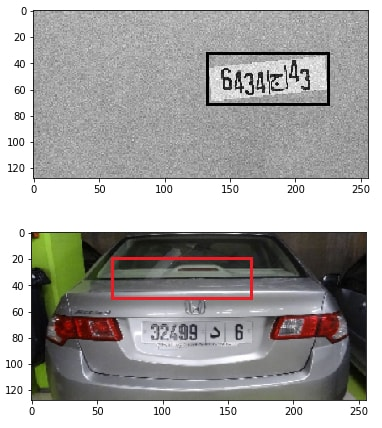
\includegraphics[width=0.7\textwidth]{figures/Resultats_1.PNG}\caption{Resultats des prédictions du réseau}
        \end{overprint}
    \end{figure}
\end{column}
\end{columns}
\end{frame}

%%%%%%%%%%%%%%%%%%%%%%%%%%%%%%%%%%%%%%%%%%%%%%%%
% Cinquième diapo
%%%%%%%%%%%%%%%%%%%%%%%%%%%%%%%%%%%%%%%%%%%%%%%%

\begin{frame}
\frametitle{Création du réseau de neurones}
\framesubtitle{Un problème de classification ?}

\begin{itemize}
    \item<1->   Problème : Dimentionnalité élevée du problème .
    %Une des solutions consiste à remplacer les données originales par des données dans un espace de plus de petite dimension, tout en conservant l'essentiel des caractéristiques de celles-ci. C'est la réduction de la dimensionnalité. Deux approches classiques sont la sélection de caractéristique, qui consiste à choisir un petit ensemble de variables représentatives, et l'extraction de caractéristique, qui consiste à définir de nouvelles variables plus pertinentes.
    \item<2->   Idée : Extraction de caractéristiques.
    \item<3->   Solution : Réseaux de neurones convolutionnels.
    \item<4->   Inconvenient : Traitement de chaque région dans l'image.
\end{itemize}

\centering
\begin{figure}
    \begin{overprint}
        \captionsetup{justification=centering}
        \onslide<1>\centering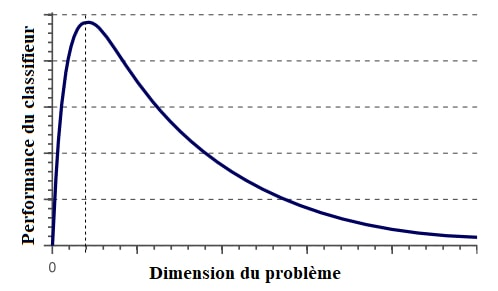
\includegraphics[width=0.55\textwidth]{figures/Malediction.PNG}\caption{Malédiction de la dimensionnalité}
        \onslide<2>\centering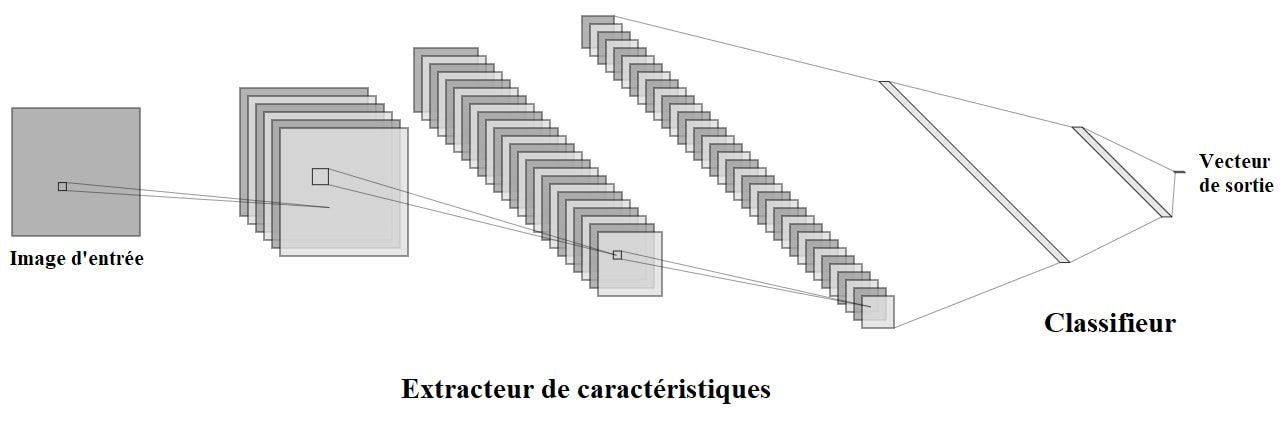
\includegraphics[width=0.95\textwidth]{figures/Extracteur.PNG}\caption{Principe de l'extraction des caracteristiques}
        \onslide<3>\centering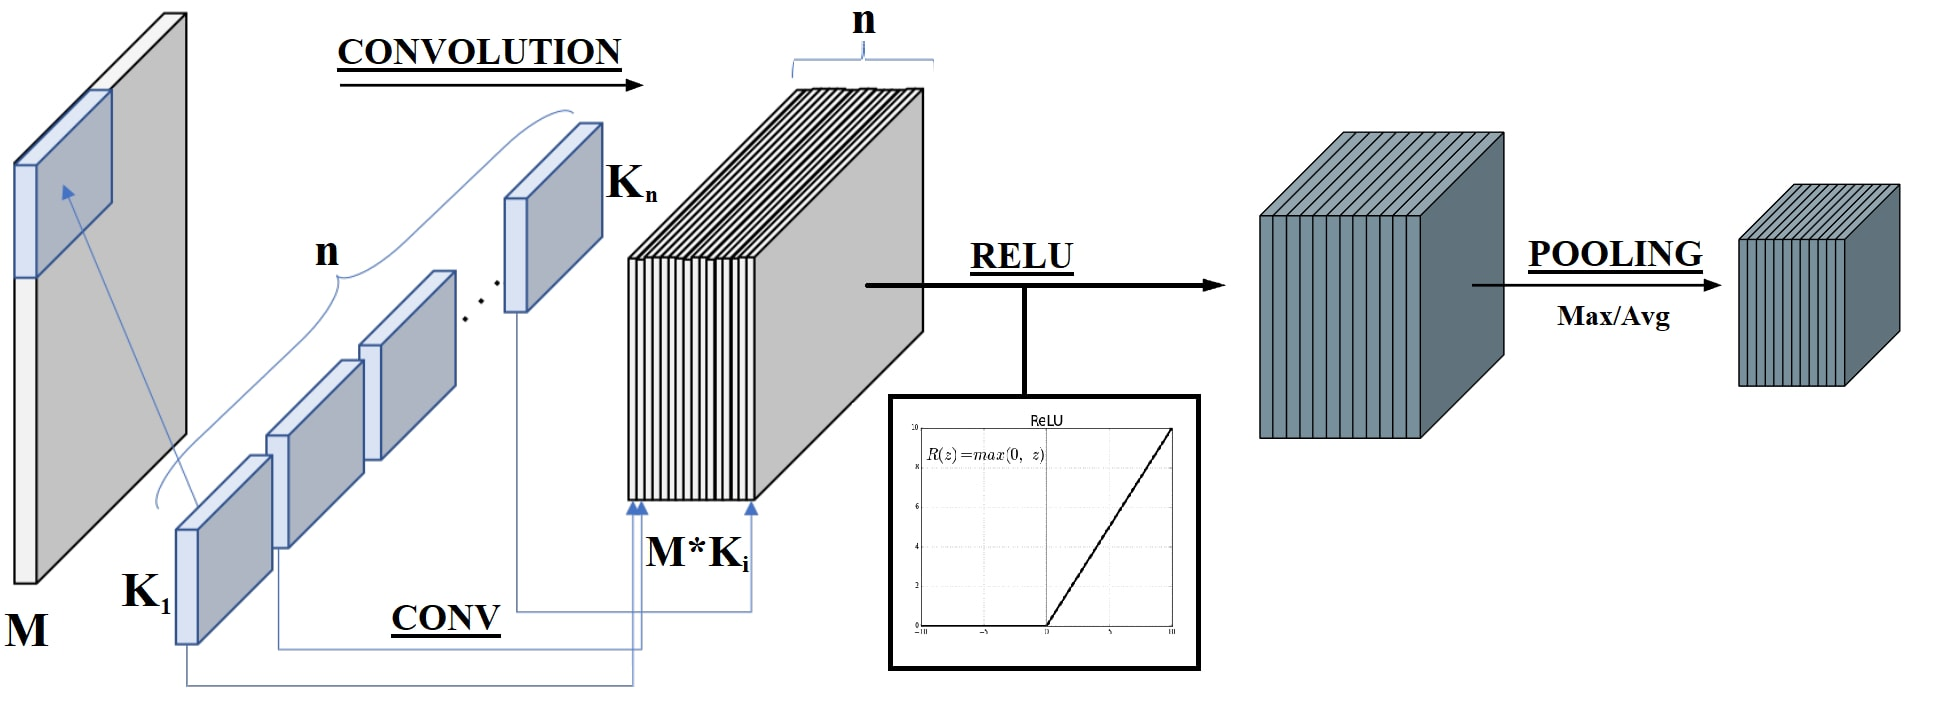
\includegraphics[width=0.85\textwidth]{figures/Conv_RELU_Pool.PNG}\caption{Principe du bloc de convolution}
        \onslide<4>\centering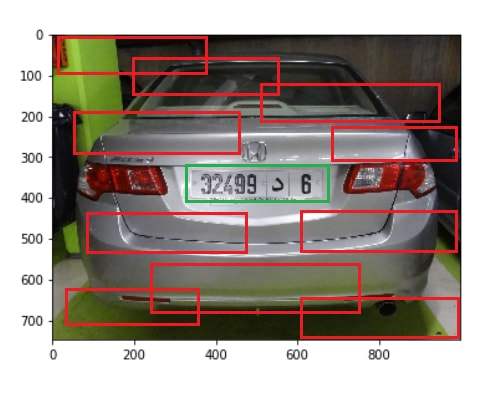
\includegraphics[width=0.37\textwidth]{figures/RCNN.PNG}\caption{Détection par fenêtres glissantes}
    \end{overprint}
\end{figure}
\end{frame}


%%%%%%%%%%%%%%%%%%%%%%%%%%%%%%%%%%%%%%%%%%%%%%%%
% Cinquième diapo
%%%%%%%%%%%%%%%%%%%%%%%%%%%%%%%%%%%%%%%%%%%%%%%%

\begin{frame}
\frametitle{Création du réseau de neurones}
\framesubtitle{Solution Optimale}


\begin{itemize}
    \item<1->   "YOLO" : Une transformation de l'espace du problème
    \begin{itemize}
        \item<2->   Diviser l'image en grilles
        \item<3->   Localiser celle contenant le centre de l'objet.
        \item<4->   Déterminer le vecteur de sortie.
    \end{itemize}
\end{itemize}

\centering
\begin{figure}
    \begin{overprint}
        \onslide<1>\centering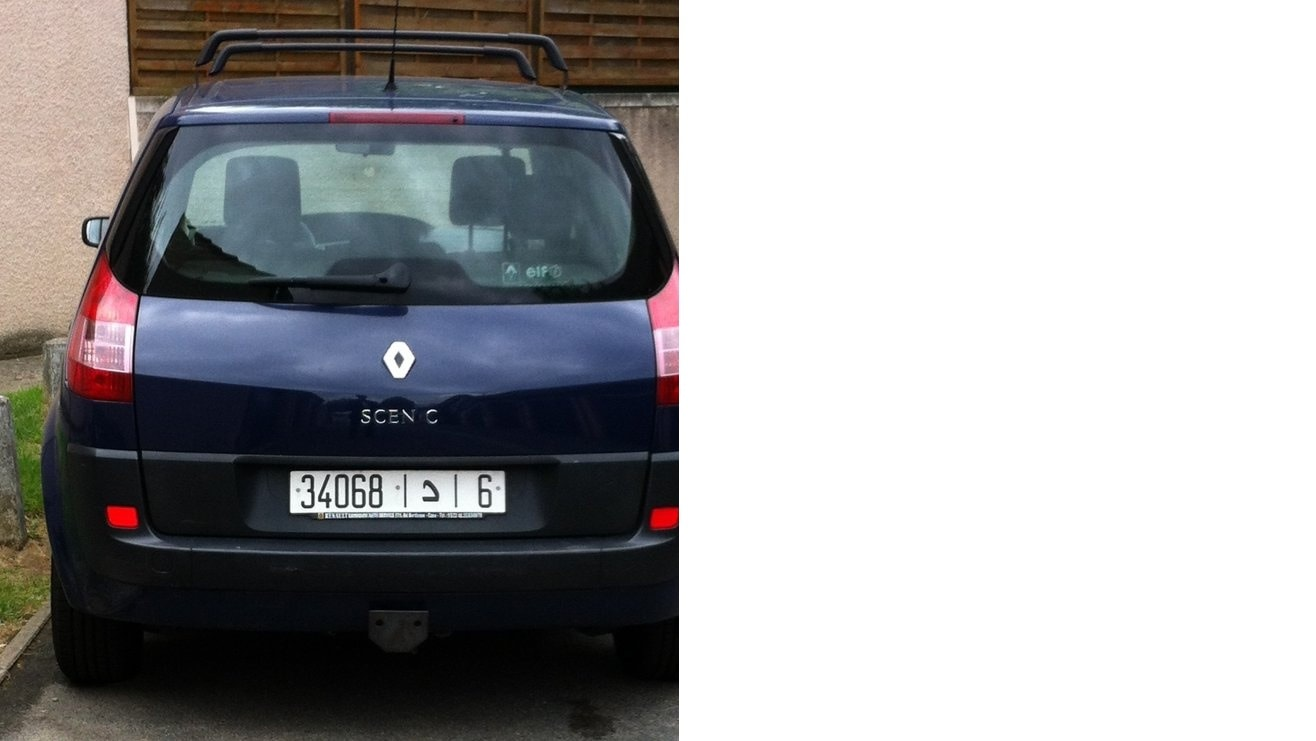
\includegraphics[width=0.6\textwidth]{figures/Car.PNG}\caption{Exemple d'image à traiter}
        \onslide<2>\centering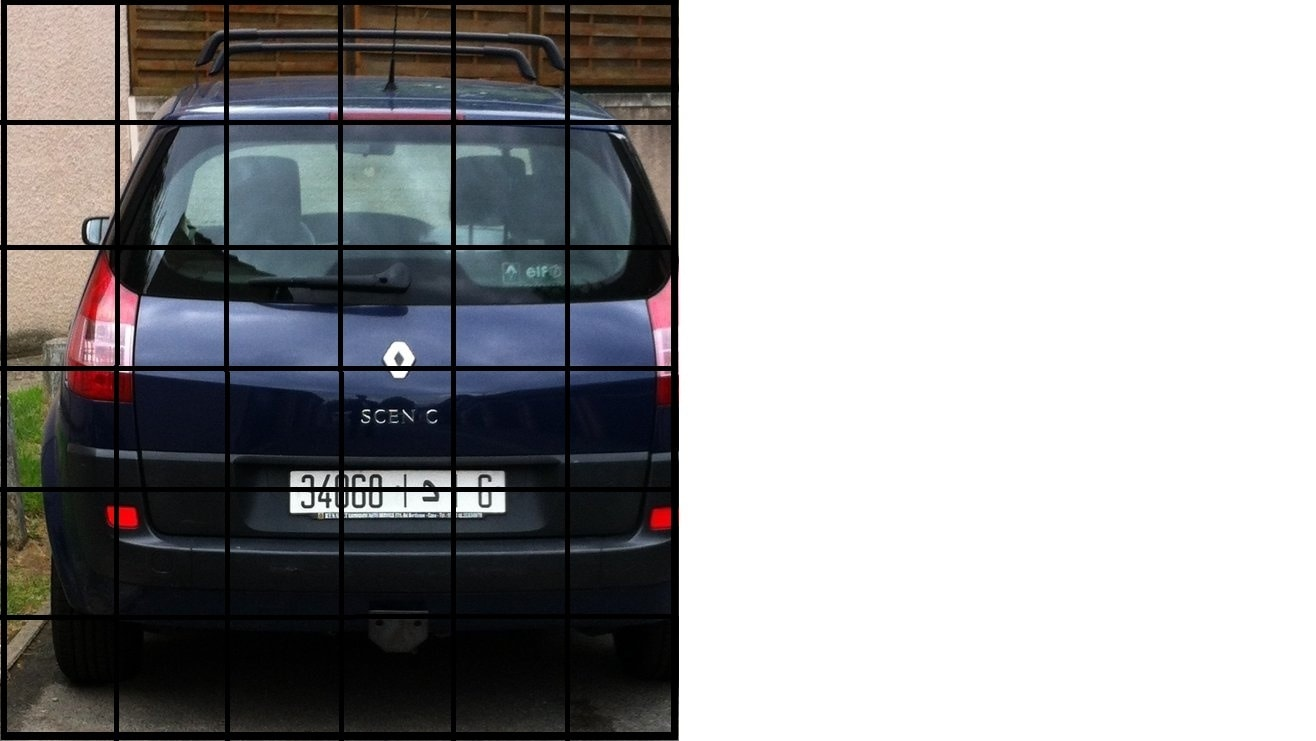
\includegraphics[width=0.6\textwidth]{figures/Grid.PNG}\caption{Première étape}
        \onslide<3>\centering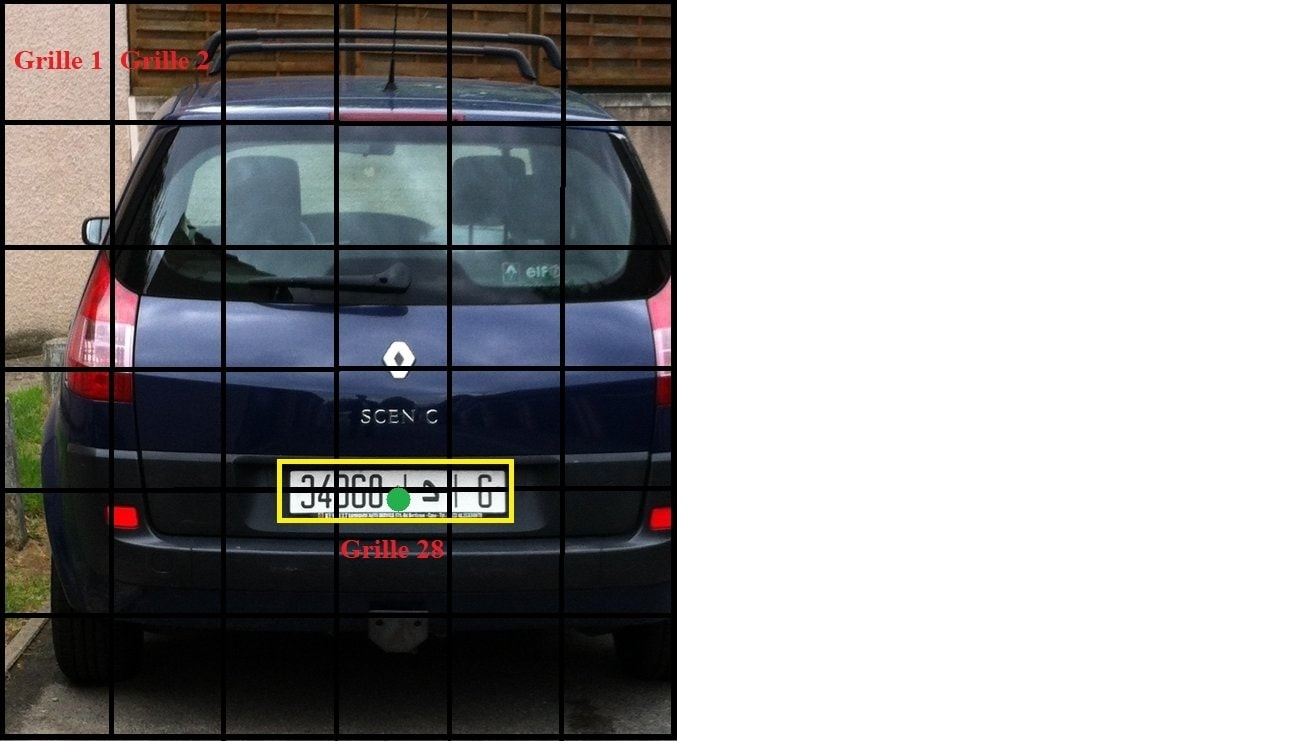
\includegraphics[width=0.6\textwidth]{figures/Center.PNG}\caption{Deuxième étape}
        \onslide<4>\centering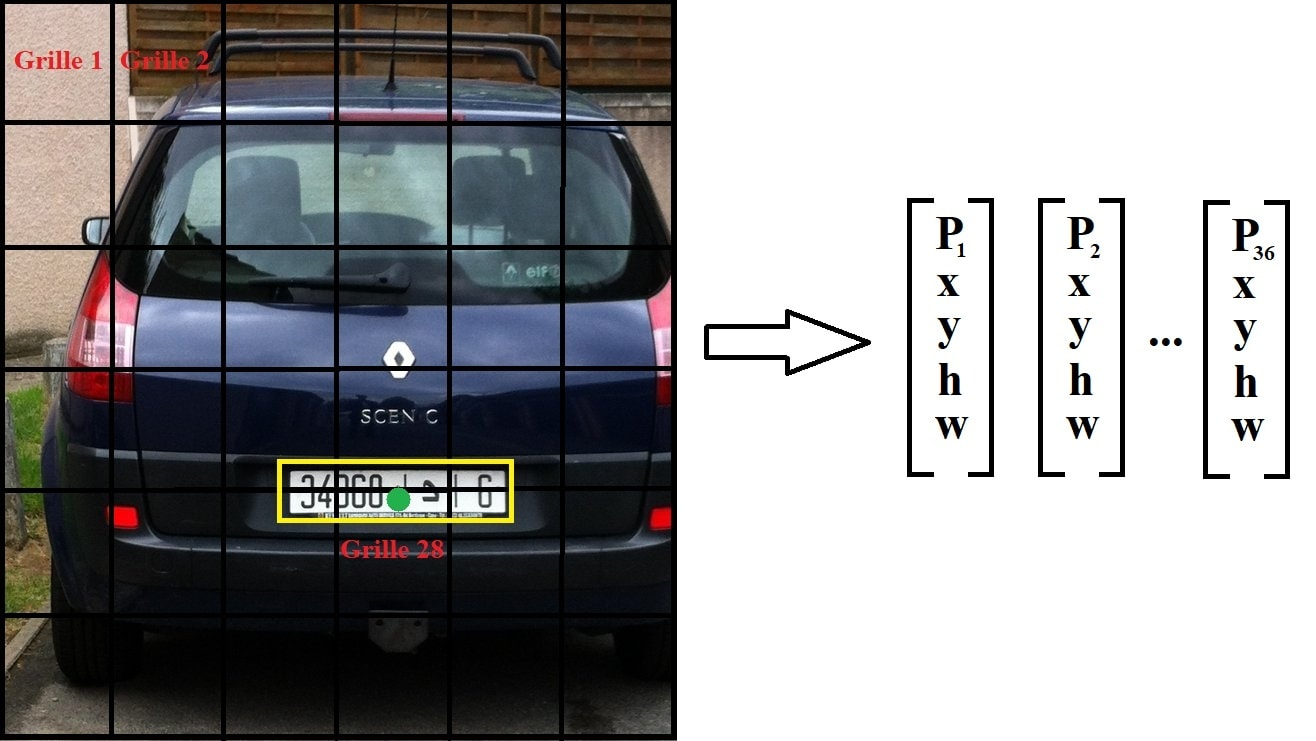
\includegraphics[width=0.6\textwidth]{figures/YOLO.PNG}\caption{Troisième étape}
    \end{overprint}
\end{figure}
\end{frame}

%%%%%%%%%%%%%%%%%%%%%%%%%%%%%%%%%%%%%%%%%%%%%%%%
% Sixième diapo
%%%%%%%%%%%%%%%%%%%%%%%%%%%%%%%%%%%%%%%%%%%%%%%%

\begin{frame}
\frametitle{Création du réseau de neurones}
\framesubtitle{Variété de solutions}

\begin{itemize}
    \item<1->   Differents extracteurs de caractéristiques :
    \begin{itemize}
        \item<1->   DarkNet : Structure originale.
        \item<2->   MobileNet : Développée par Google.
        \item<3->   SqueezeNet : Développée par Stanford.
    \end{itemize}
\end{itemize}
\begin{figure}
    \begin{overprint}
        \onslide<1>\centering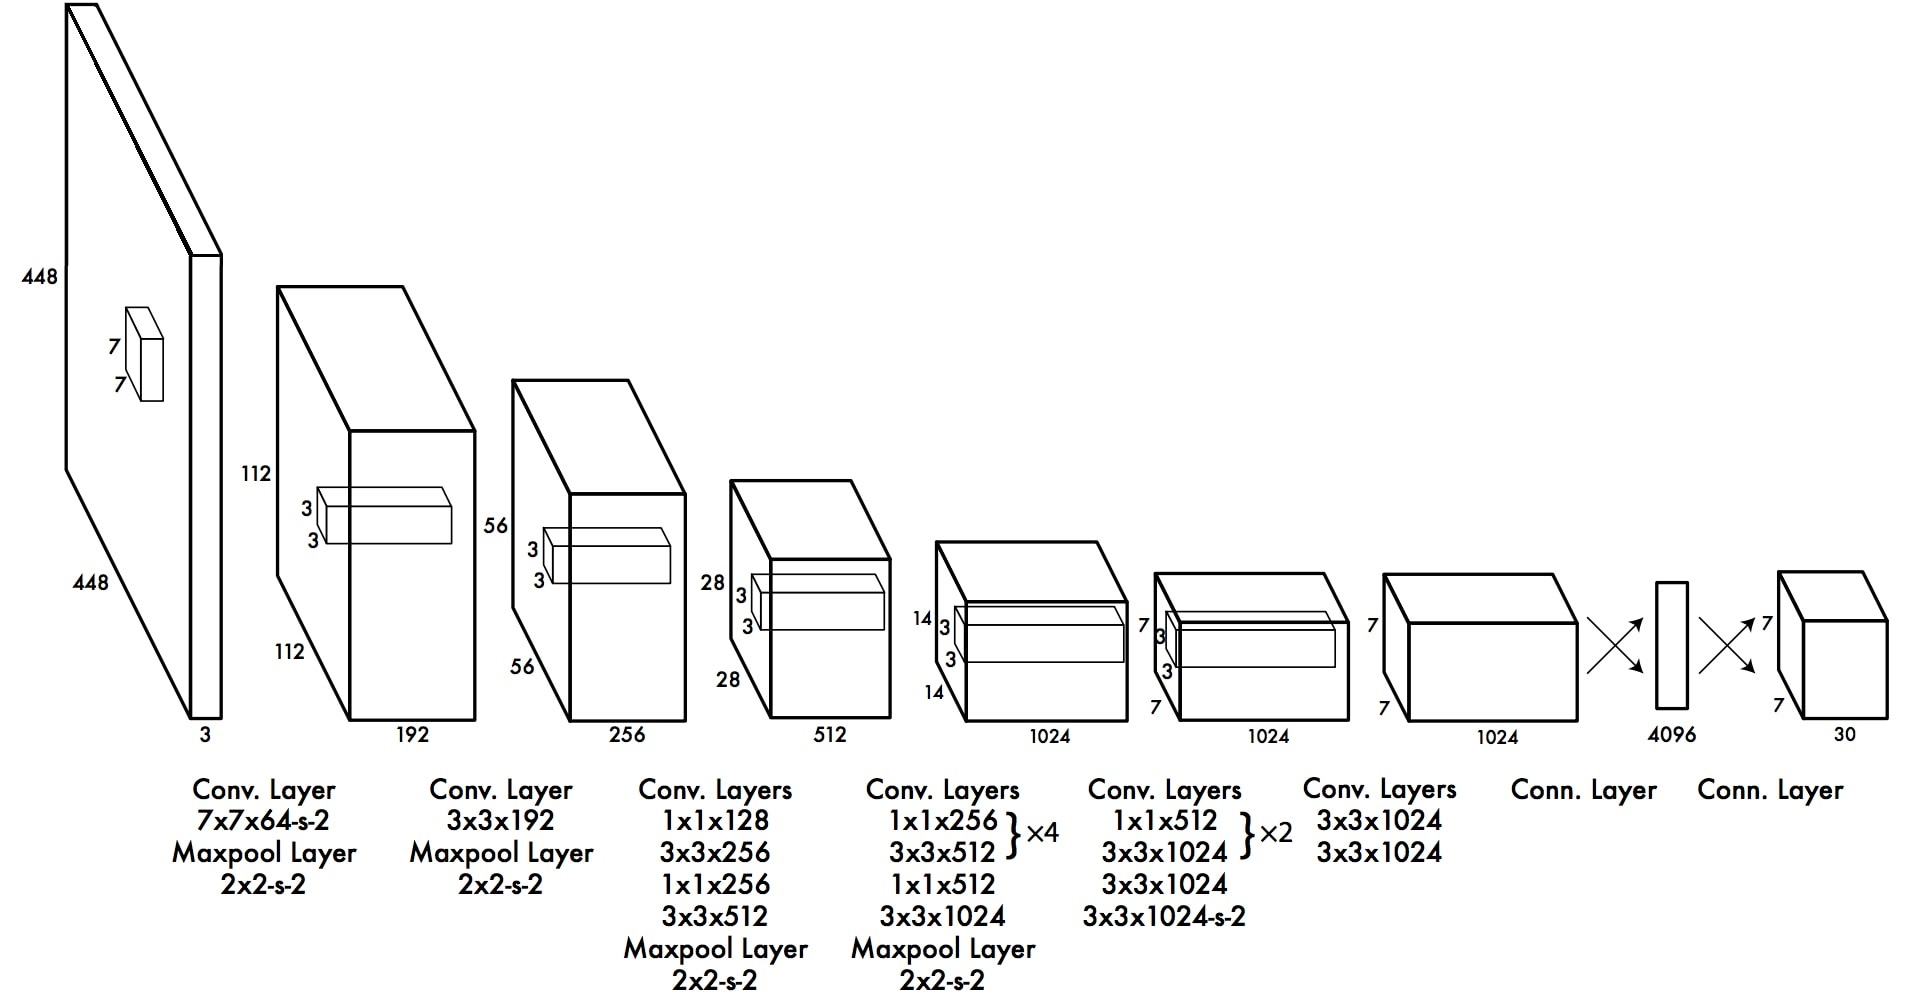
\includegraphics[width=0.67\textwidth]{figures/Darknet.PNG}\caption{Structure globale de DarkNet}
        \onslide<2>\centering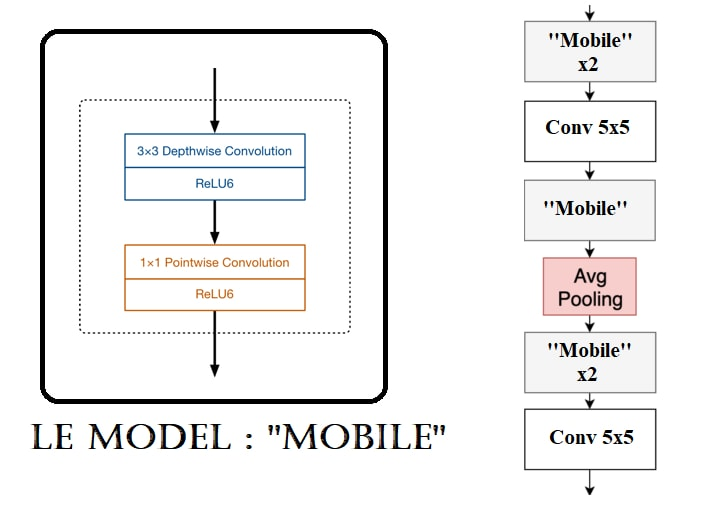
\includegraphics[width=0.45\textwidth]{figures/MobNet.PNG}\caption{Unité principale de MobileNet}
        \onslide<3>\centering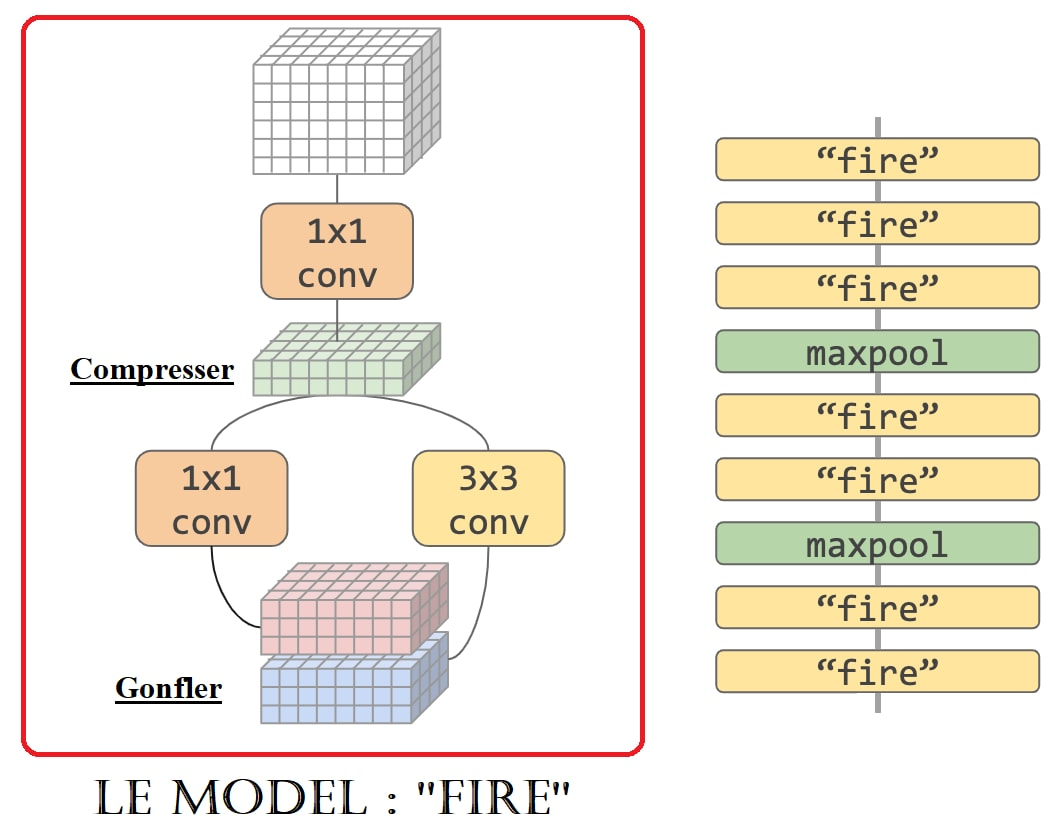
\includegraphics[width=0.42\textwidth]{figures/SqzNet.PNG}\caption{Unité principale de SqueezeNet}
    \end{overprint}
\end{figure}
\end{frame}

%%%%%%%%%%%%%%%%%%%%%%%%%%%%%%%%%%%%%%%%%%%%%%%%
% Septième diapo
%%%%%%%%%%%%%%%%%%%%%%%%%%%%%%%%%%%%%%%%%%%%%%%%

\begin{frame}
\frametitle{Création du réseau de neurones}
\framesubtitle{Comparaison entre structures}

\begin{table}
\begin{tabular}{c|c|c|c}
    Classifieur  &  Nombre de   &  Temps de    &  Temps          \\
                 &  paramètres  &  traitement  &  d'entrainement \\
    \hline
    DarkNet      &  50,983,561  &  0.5  s      &  Plus que 20 jours \\
    MobileNet    &  3,284,214   &  0.09 s      &  6 jours et 3 heures  \\
    SqueezeNet   &  750,198     &  0.02 s      &  1 jours et 14 heures
\end{tabular}
\end{table}
\centering
\begin{figure}
    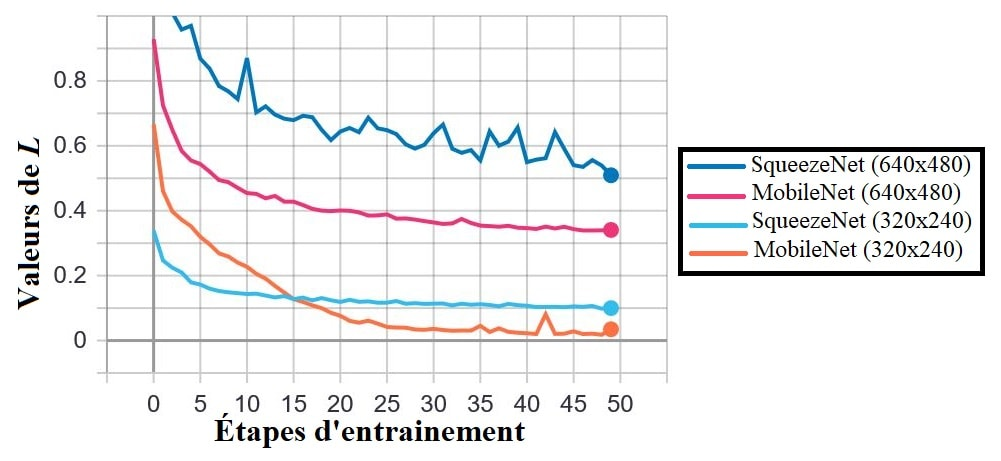
\includegraphics[width=0.55\textwidth]{figures/Epochs.PNG}\caption{Resultats d'entrainement}
\end{figure}
\end{frame}

%%%%%%%%%%%%%%%%%%%%%%%%%%%%%%%%%%%%%%%%%%%%%%%%
% huitième diapo
%%%%%%%%%%%%%%%%%%%%%%%%%%%%%%%%%%%%%%%%%%%%%%%%

\begin{frame}
\frametitle{Création du réseau de neurones}
\framesubtitle{Évaluation de la structure retunue : SqueezeNet}
\captionsetup{justification=centering}
\begin{columns}
\begin{column}{6cm}
    \begin{itemize}
    \item<1->   Sur les images :
    \begin{itemize}
        \item<1->   Bons résultats.
        \item<1->   Bonus : Généralisation.
    \end{itemize}
    \item<2->   Sur un flux vidéo :
        \begin{itemize}
            \item<2->   Détection en temps réel.
            \item<2->   Bonus : Multi-détection.
        \end{itemize}
    \end{itemize}
\end{column}
\begin{column}{6cm}
    \begin{figure}
        \begin{overprint}
        \captionsetup{justification=centering}
            \onslide<1>\centering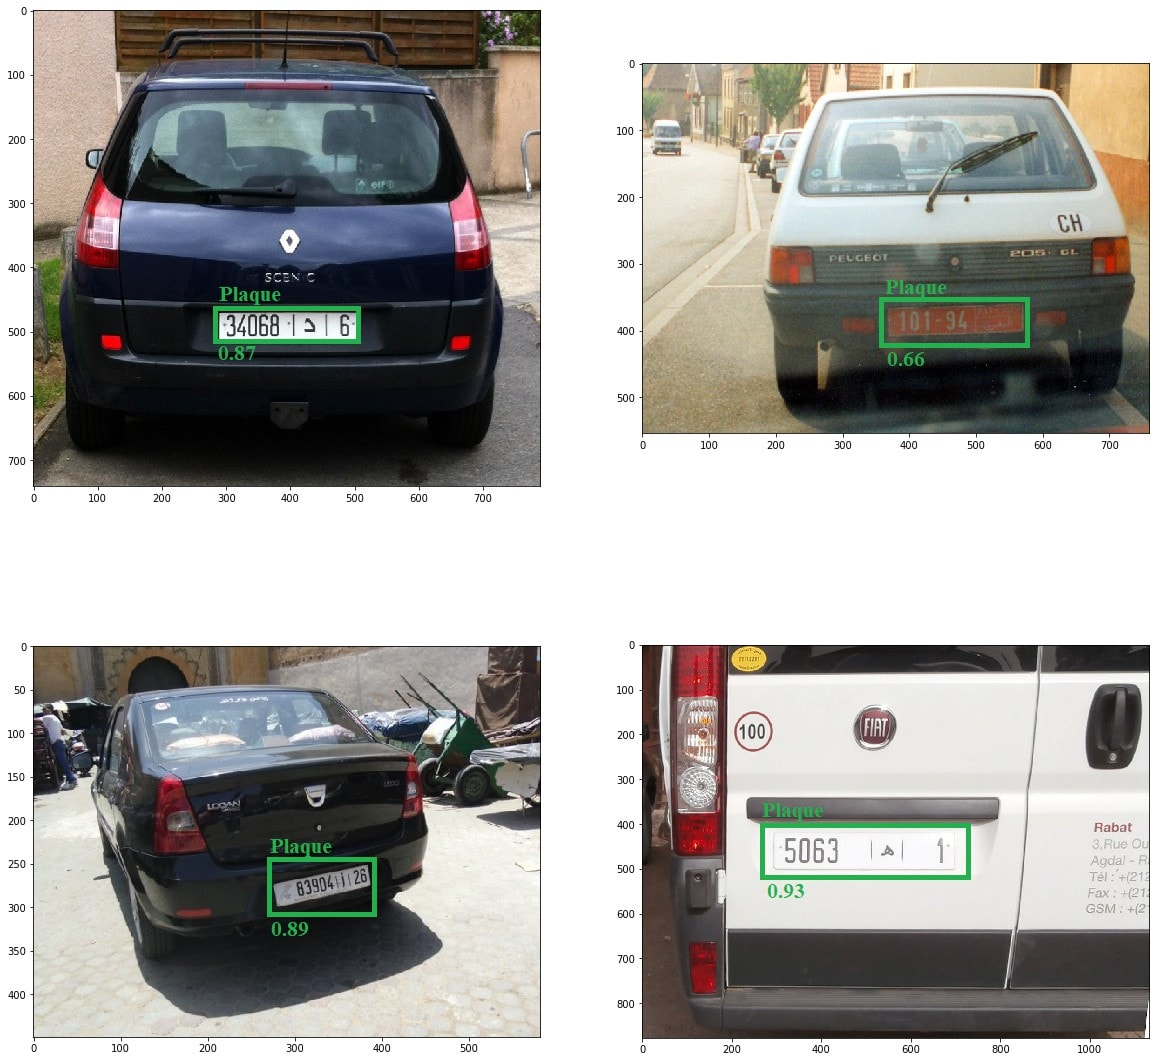
\includegraphics[width=0.8\textwidth]{figures/Eval.PNG}\caption{Exemples de détections dans des cas differents}
            \onslide<2>\centering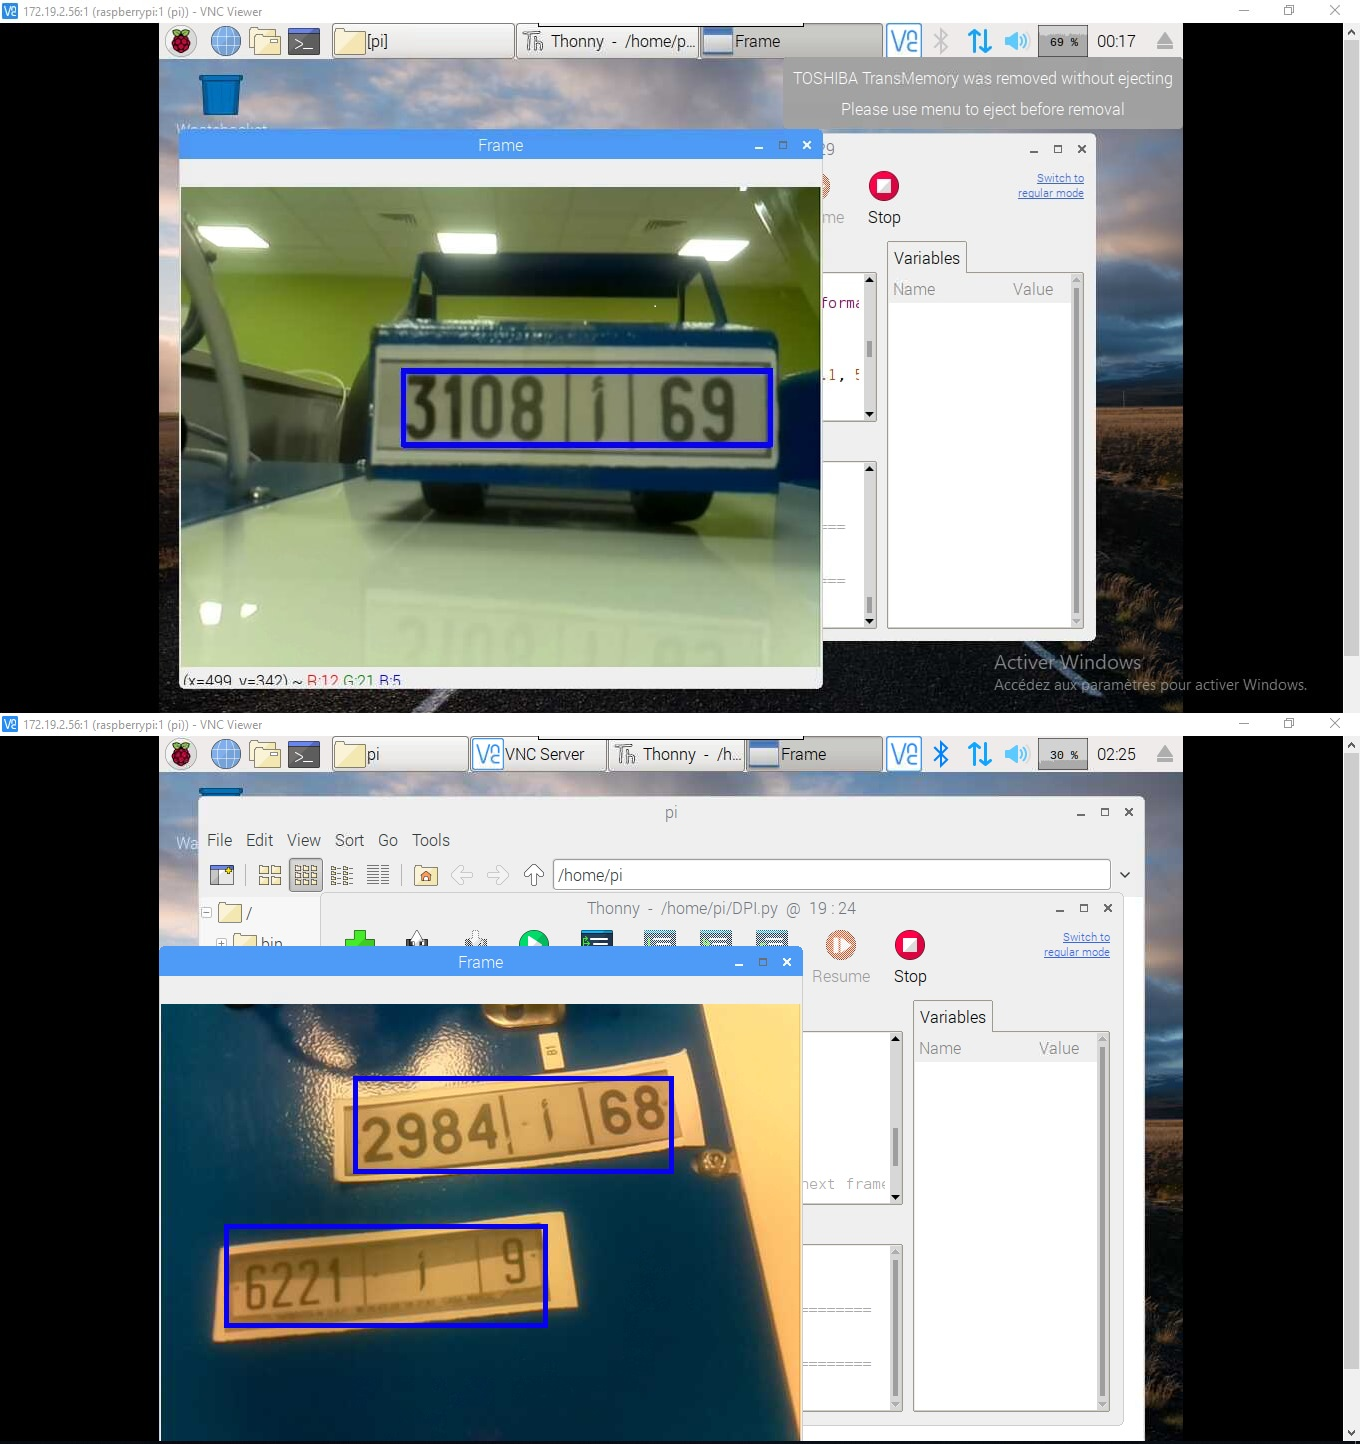
\includegraphics[width=0.8\textwidth]{figures/Stream.PNG}\caption{Resultats avec Raspberry}
        \end{overprint}
    \end{figure}
\end{column}
\end{columns}
\end{frame}

% Réalisation
\section{Réalisation et implémentation}

%%%%%%%%%%%%%%%%%%%%%%%%%%%%%%%%%%%%%%%%%%%%%%%%
% Première diapo
%%%%%%%%%%%%%%%%%%%%%%%%%%%%%%%%%%%%%%%%%%%%%%%%

\begin{frame}
\frametitle{Un système embarqué}
\framesubtitle{Circuit de commande}

\begin{figure}
    \centering
    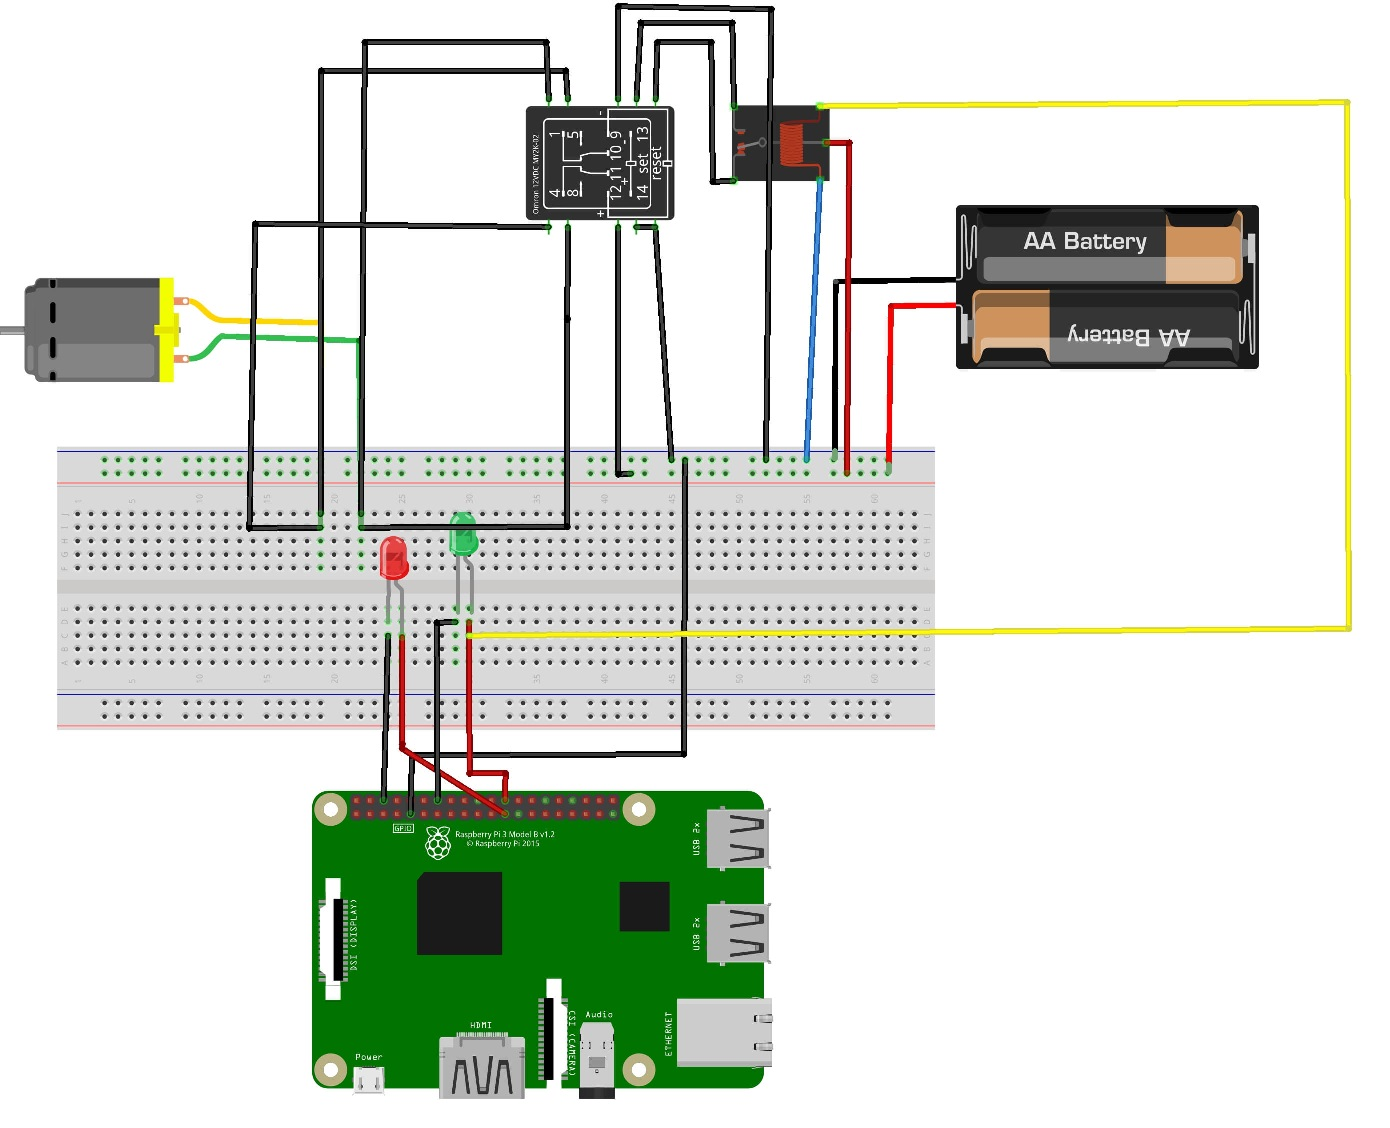
\includegraphics[width=0.5\textwidth]{figures/Montage1.jpg}\caption{Montage de commande}
\end{figure}

\end{frame}

%%%%%%%%%%%%%%%%%%%%%%%%%%%%%%%%%%%%%%%%%%%%%%%%
% Deuxième diapo
%%%%%%%%%%%%%%%%%%%%%%%%%%%%%%%%%%%%%%%%%%%%%%%%

\begin{frame}
\frametitle{Un système embarqué}
\framesubtitle{Experimentation finale}

\begin{columns}
    \begin{column}{6cm}
        \begin{figure}
            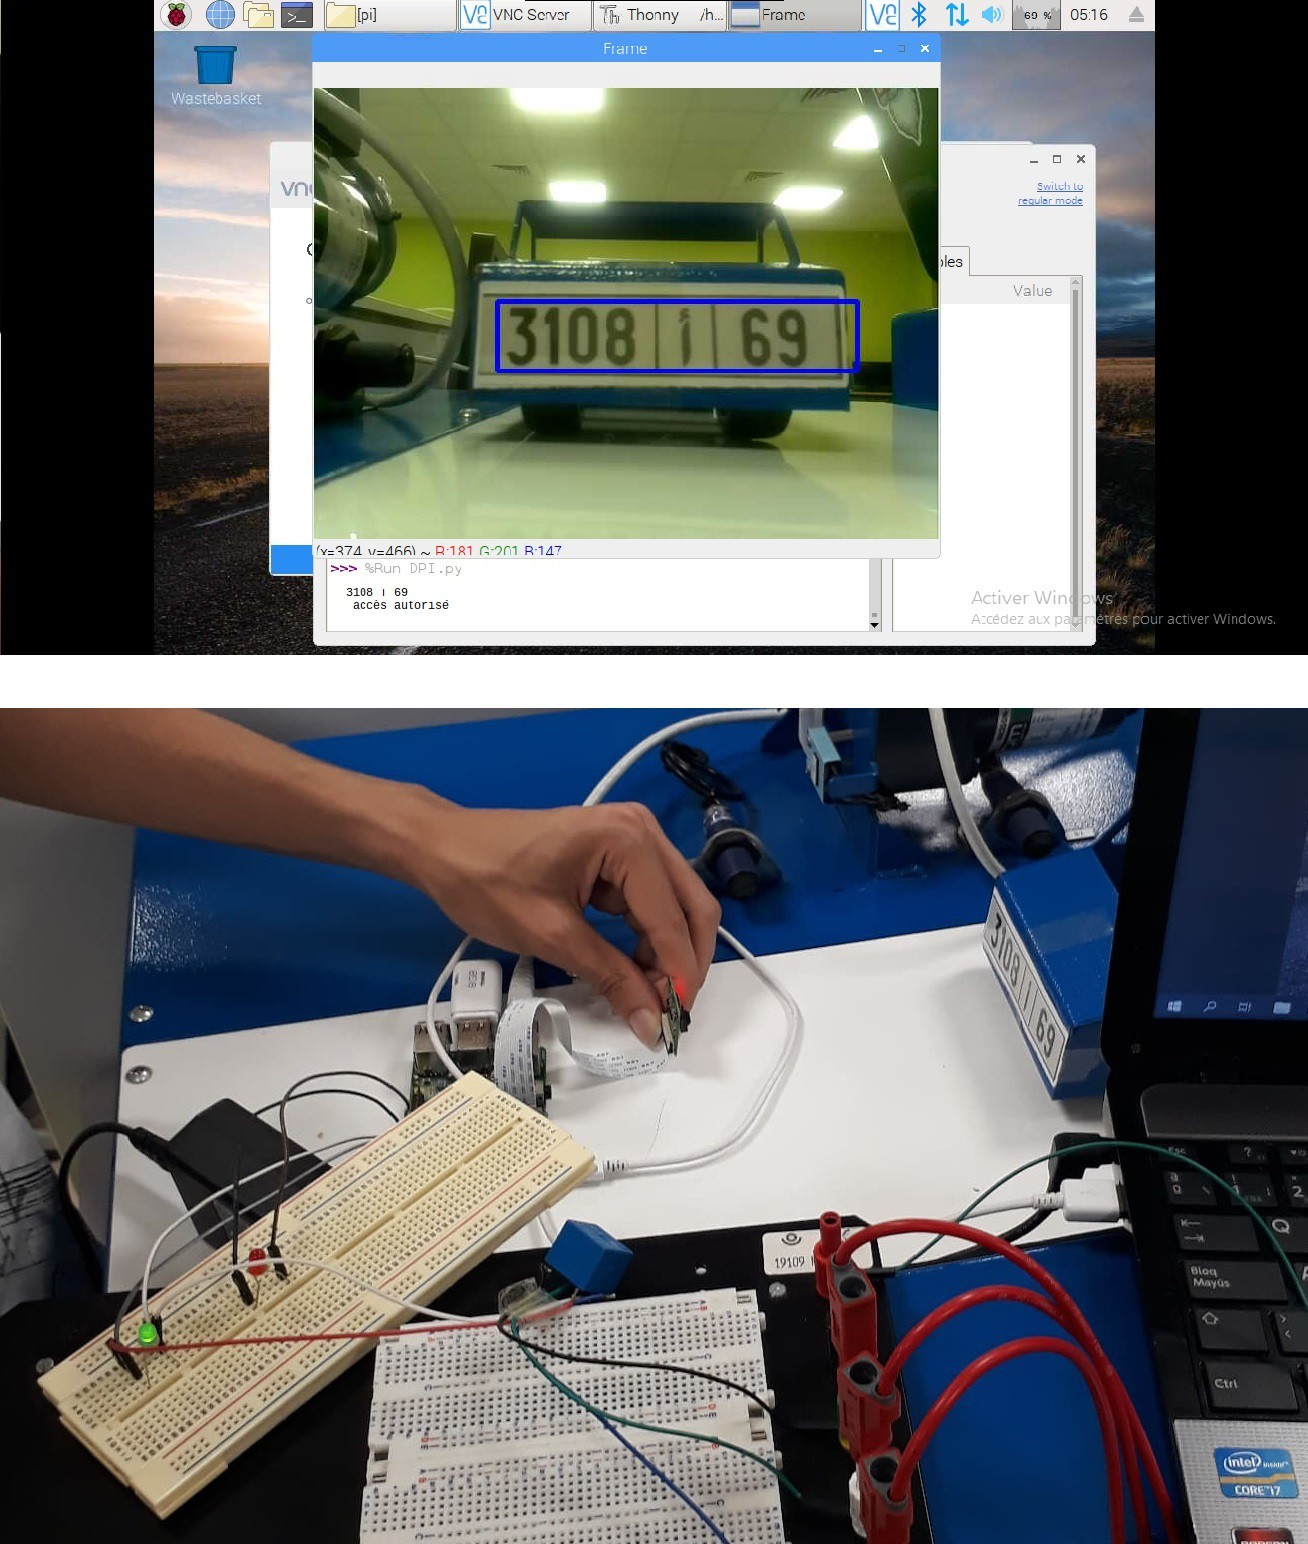
\includegraphics[width=0.6\textwidth]{figures/Autorise.jpg}\caption{Essaie sur une plaque autorisée}
        \end{figure}
    \end{column}
    \begin{column}{6cm}
        \begin{figure}
            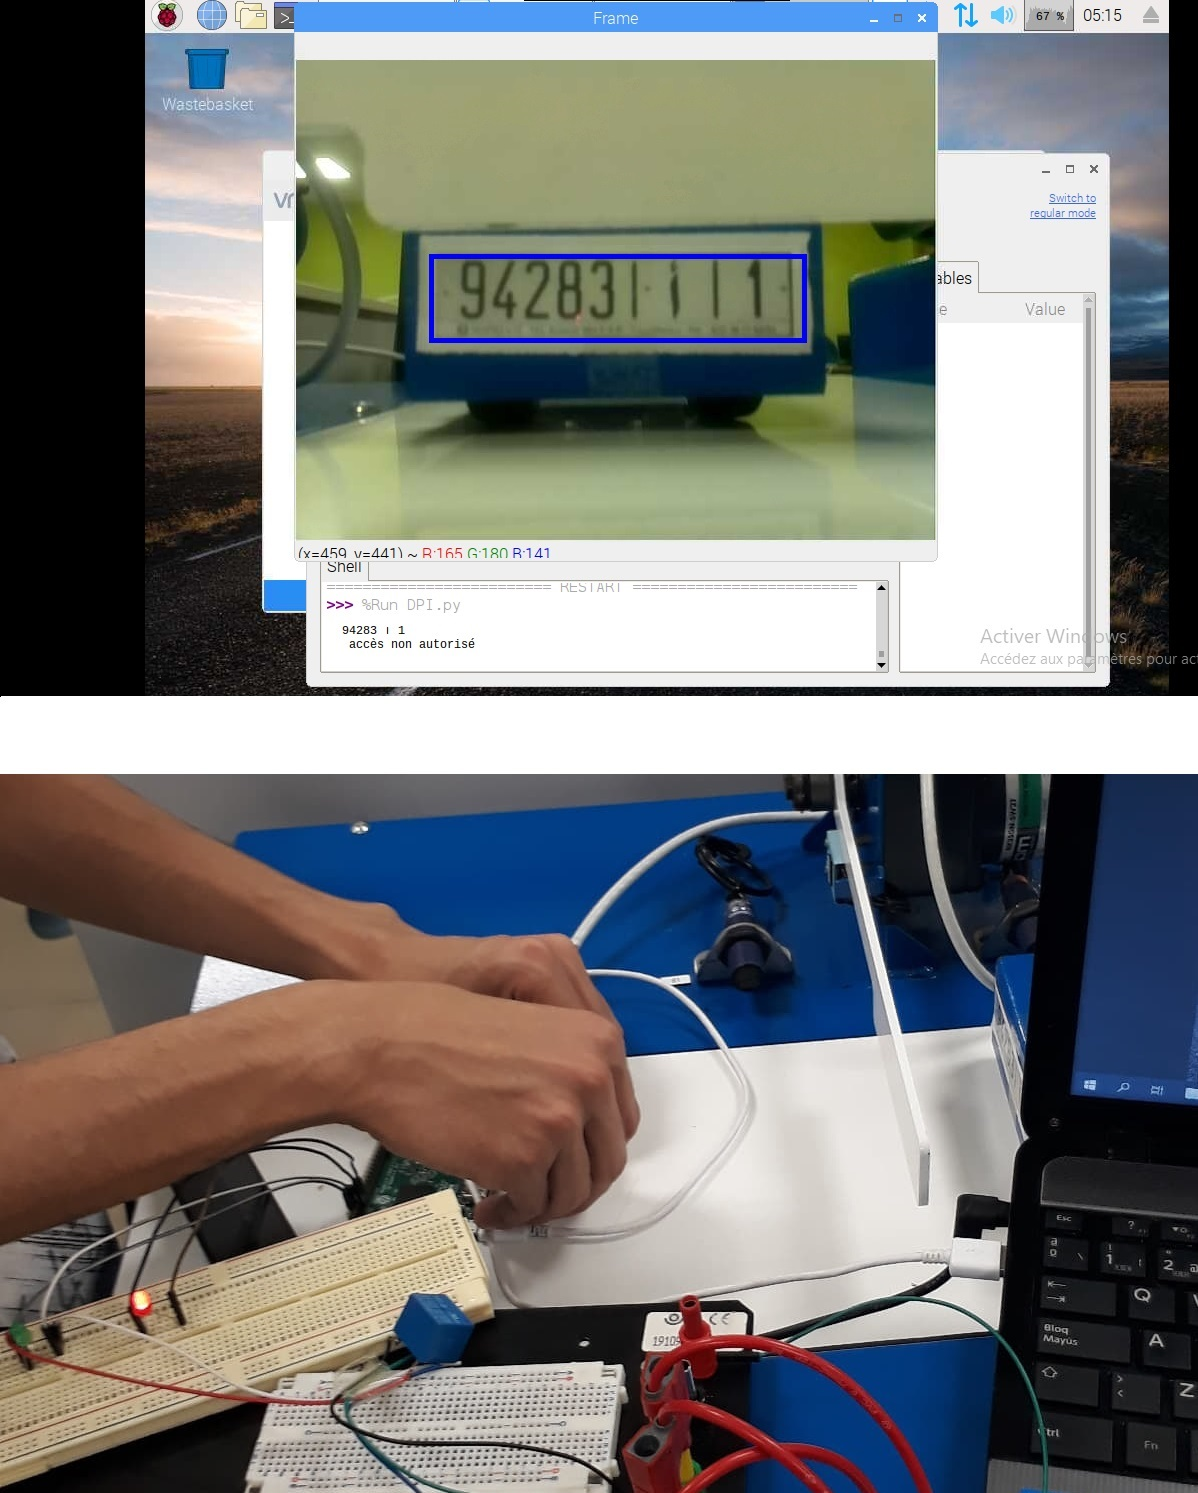
\includegraphics[width=0.6\textwidth]{figures/Refuse.jpg}\caption{Essaie sur une plaque non autorisée}
        \end{figure}
    \end{column}
\end{columns}
\end{frame}


%%%%%%%%%%%%%%%%%%%%%%%%%%%%%%%%%%%%%%%%%%%%%%%%
% Deuxième diapo
%%%%%%%%%%%%%%%%%%%%%%%%%%%%%%%%%%%%%%%%%%%%%%%%


% Conclusion
\section{Conclusion}

\begin{frame}
\frametitle{Conclusion}
%\framesubtitle{}

\begin{itemize}
    \item<1->    Les réseaux de neurones sont puissants
    \begin{itemize}
        \item<1->    Etat de l'art dans plusieurs domaines;
        \item<1->    Peuvent encore être développés;
    \end{itemize}
    
    \item<1->    Pourtant ...
    \begin{itemize}
        \item<1->    Ils sont trés compliqués à implémenter;
        \item<1->    Difficulté de les entrainer;
    \end{itemize}
\end{itemize}
\end{frame}

\begin{frame}

\begin{center}
{\fontsize{100}{100}\selectfont Merci pour votre attention!}
\end{center}

\end{frame}

\end{document}


